\documentclass[9pt,t]{beamer} %it is important to use 9pt fontsize as everithing is set up to this size

%%% Set theme %%%
\usetheme{Dingo} %using Dingo theme

%%% Import required minimum packages %%%
\usepackage{lipsum}
\usepackage[utf8]{inputenc}
\usepackage{pgf}
\usepackage{booktabs}
\usepackage{xltxtra}
\usepackage{xeCJK}
\usepackage{braket}
\usepackage{graphicx,caption}
\usepackage{extarrows}
\graphicspath{{figures/}}
\usepackage{color}
\setCJKmainfont[BoldFont={SimHei}]{SimSun}
\setCJKsansfont{SimSun} % Sorry I don't have enough fonts.
\setCJKmonofont{SimHei}

% \setCJKmainfont[BoldFont=Adobe Heiti Std,ItalicFont=Adobe Kaiti Std]{Adobe Song Std}
% \setCJKsansfont{Adobe Heiti Std}
% \setCJKmonofont{Adobe Fangsong Std}
% \setCJKfamilyfont{song}{Adobe Song Std}
% \setCJKfamilyfont{hei}{Adobe Heiti Std}
% \setCJKfamilyfont{fangsong}{Adobe Fangsong Std}
% \setCJKfamilyfont{kai}{Adobe Kaiti Std}

\punctstyle{quanjiao}
% \usepackage{zhspacing}
% \zhspacing
\setbeamercolor{institute}{fg=black}		%institute color
\setbeamercolor{normal text}{fg = black}	%text color
\setbeamercolor{item}{fg=black}		%item color
\setbeamercolor{subitem}{fg=black}		%subitem color
\setbeamercolor{text}{fg=black,bg=DINGO_gray}		%text block color
\setbeamercolor{block title}{bg=DINGO_gray,fg=white}		%block title color
\setbeamercolor{block body}{bg=DINGO_lightgray,fg=black} %block body color
\setbeamercolor{foot}{fg=white}        %only fontsize needed if there is a background picture
\setbeamerfont{frametitle}{size = \huge}			%frame title font size
\setbeamerfont{normal text}{size = \normalsize}			%text font size
\AtBeginDocument{\usebeamerfont{normal text}}
\usebeamercolor*{normal text}
%%%%%%%%%%%%%%%%%%%%%%%%%%%%%%%%%%%%%%%%%%%%%%%%%%%%%%%%%%%%%%%%%
% ----------------------------------------------------------------
\vfuzz2pt % Don't report over-full v-boxes if over-edge is small
\hfuzz2pt % Don't report over-full h-boxes if over-edge is small
% ----------------------------------------------------------------
%%%%%%%%%%%%%%%%%%%%%%%%%%%%%%%%%%%%%%%%%%%%%%%%%%%%%%%%%%%%%%%%%%
%%% Tittlepage setup %%%
%%%%%%%%%%%%%%%%%%%%%%%%%%%%%%%%%%%%%%%%%%%%%%%%%%%%%%%%%%%%%%%%%%
\title[交叉学科中心]{\ \\ \ \\ 
铁磁石墨烯中的近藤效应\\ 
\Large{Kondo effect in ferromagnetic graphene}
}
% \subtitle[LaTeX for slide]{使用\LaTeX{}输出幻灯片}
\author[李高阳]{
\ \\ 
李高阳}
% \institute[Douban.com]{豆瓣\TeX{}小组}
\date{2020年8月24日}

%%% Titlepage %%%
\begin{document}

\begin{frame}[plain,t]
\normalsize
\titlepage
\end{frame}
%%%%%%%%%%%%%%%%%%%%%%%%%%%%%%%%%%%%%%%%%%%%%%%%%%%%%%%%%%%%%%%%%%
%%% Presentation body %%%
%%%%%%%%%%%%%%%%%%%%%%%%%%%%%%%%%%%%%%%%%%%%%%%%%%%%%%%%%%%%%%%%%%
\addtocounter{framenumber}{-1}  %the next frame will start from number 1 instead of 2
%%%%%%%%%%%%%%%%%%%%%%%%%%%%%%%%%%%%%%%%%%%%%%%%%%%%%%%%%%%%%%%%%%
\title{目录}
\begin{frame}{目录}
\tableofcontents
\end{frame}
%%%%%%%%%%%%%%%%%%%%%%%%%%%%%%%%%%%%%%%%%%%%%%%%%%%%%%%%%%%%%%%%%%
% \section{0.个人基本情况介绍}
% \title{个人基本情况介绍}
% \begin{frame}[t]{个人基本情况}
% \normalsize
% \begin{itemize}
% \item 教育经历
% % \textbf{兰州大学}
% \begin{itemize}
% \item[·] \textbf{兰州大学}\qquad\qquad 硕博连读与中科院兰州近物所联合培养博士\qquad\qquad (2013 -- 2019)\\
% 专业:物理学$\cdot$ 理论物理\\
% 方向:凝聚态理论\\
% 导师:罗洪刚教授(长江学者)、房铁峰教授\\
% 研究内容:强关联量子系统的数值重整化群研究\\
% 研究方法:全密度矩阵数值重整化群(数值方法)\\
% \item[·] \textbf{兰州大学}\qquad\qquad 本科\qquad\qquad\qquad\qquad\qquad\qquad\qquad\qquad\qquad\qquad\quad (2009 --  2013)\\
% 专业:物理学国家基地班
% \end{itemize}
% \\
% \item 发表文章
% \begin{itemize}
% \item[·] \textbf{Gao-Yang Li}, Tie-Feng Fang, Ai-Min Guo, and Qing-Feng Sun \textit{Ferromagnetism-induced Kondo effect in graphene with a magnetic impurity}, Phys. Rev. B \textbf{100}, 115115 (2019).
% \item[·] Wan-Xiu He, Zhan Cao, \textbf{Gao-Yang Li}, Lin Li, Hai-Feng Lü, ZhenHua Li, and Hong-Gang Luo \textit{Performance of the T-matrix based master equation for Coulomb drag in double quantum dots}, Phys. Rev. B \textbf{101}, 035417 (2020).
% \end{itemize}
% \\
% \item 获奖情况
% \begin{itemize}
% \item[·] 国家励志奖学金\hspace{6.5cm} (2010 -- 2011)
% % \item[·] 学校三等奖学金\hspace{6.5cm} (2013 -- 2018)
% \end{itemize}
% \end{itemize}
% \end{frame}

\section{1.研究背景及研究方法}
% \subsection{1.1量子杂质系统}

\begin{frame}
\tableofcontents[currentsection] 
\end{frame}

% \title{铁磁石墨烯中近藤效应的NRG研究 \qquad \qquad 什么样的系统中可以现出近藤效应?}
% \begin{frame}[t]{量子杂质系统}
% % \small
% \begin{minipage}[t]{0.25 \textwidth}
% \begin{figure}
% \centering
% 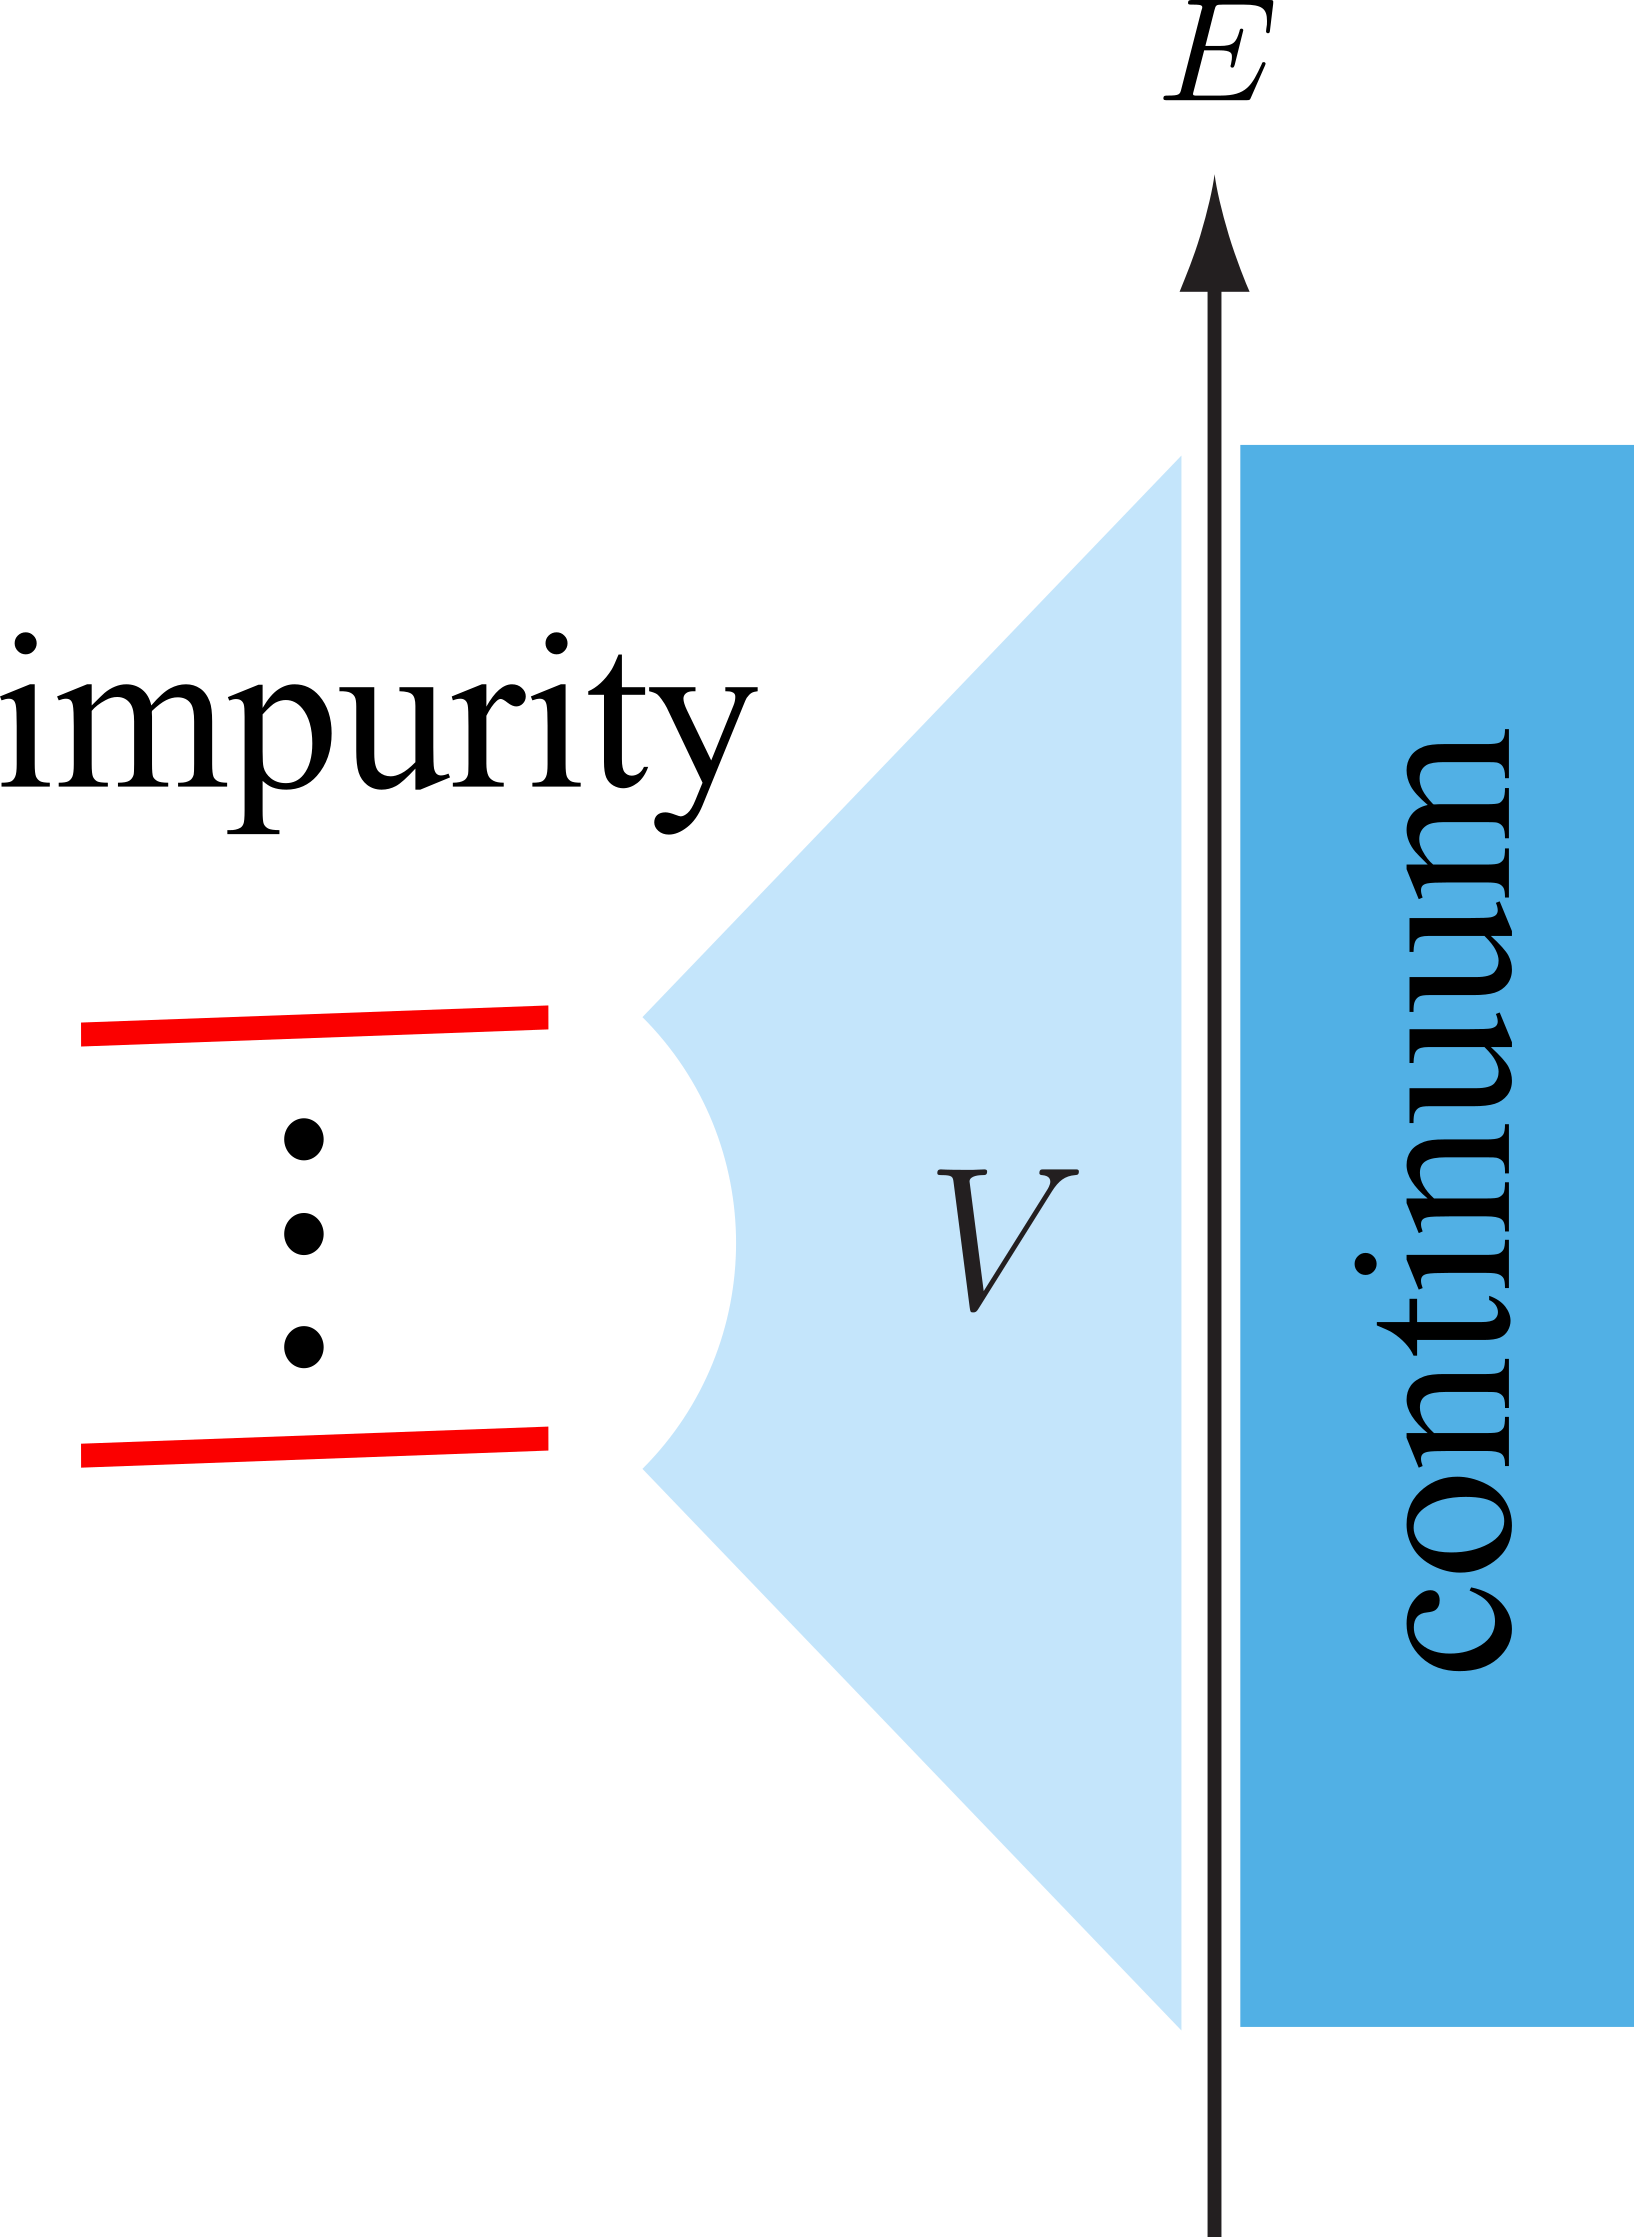
\includegraphics[width=0.9\textwidth]{QIP.png}
% \end{figure}
% \end{minipage}%
% \begin{minipage}[t]{0.75 \textwidth}
% \ \\
% 模型哈密顿量:\\
% \text{\ } $\quad \qquad$ $H=H_{\rm{imp}}+H_{\rm{bath}}+H_{\rm{imp-bath}}$
% \begin{itemize}
% \setlength\itemsep{0.7em}
% \item 有少量内禀自由度的杂质(磁性杂质、量子点、二能级原子,如$H_{\rm{imp}}=\sum_{i\sigma}\varepsilon_{i\sigma}d_{i\sigma}^{\dag}d_{i\sigma}$)
% \item 连续能带(金属中费米型的传导电子、玻色型的集体激发,如$H_{\rm{bath}}=\sum_{k\sigma}\varepsilon_{k\sigma}c_{k\sigma}^{\dag}c_{k\sigma}$)
% % \item 区别于格点问题(整个系统的状态往往取决于局域化的杂质的状态)
% % \item 数值重整化群(Numerical renormalization group)
% \item 检验多体理论、为器件应用提供理论基础
% \end{itemize}
% \end{minipage}\\ $\quad$
% \begin{figure}
% \centering
% 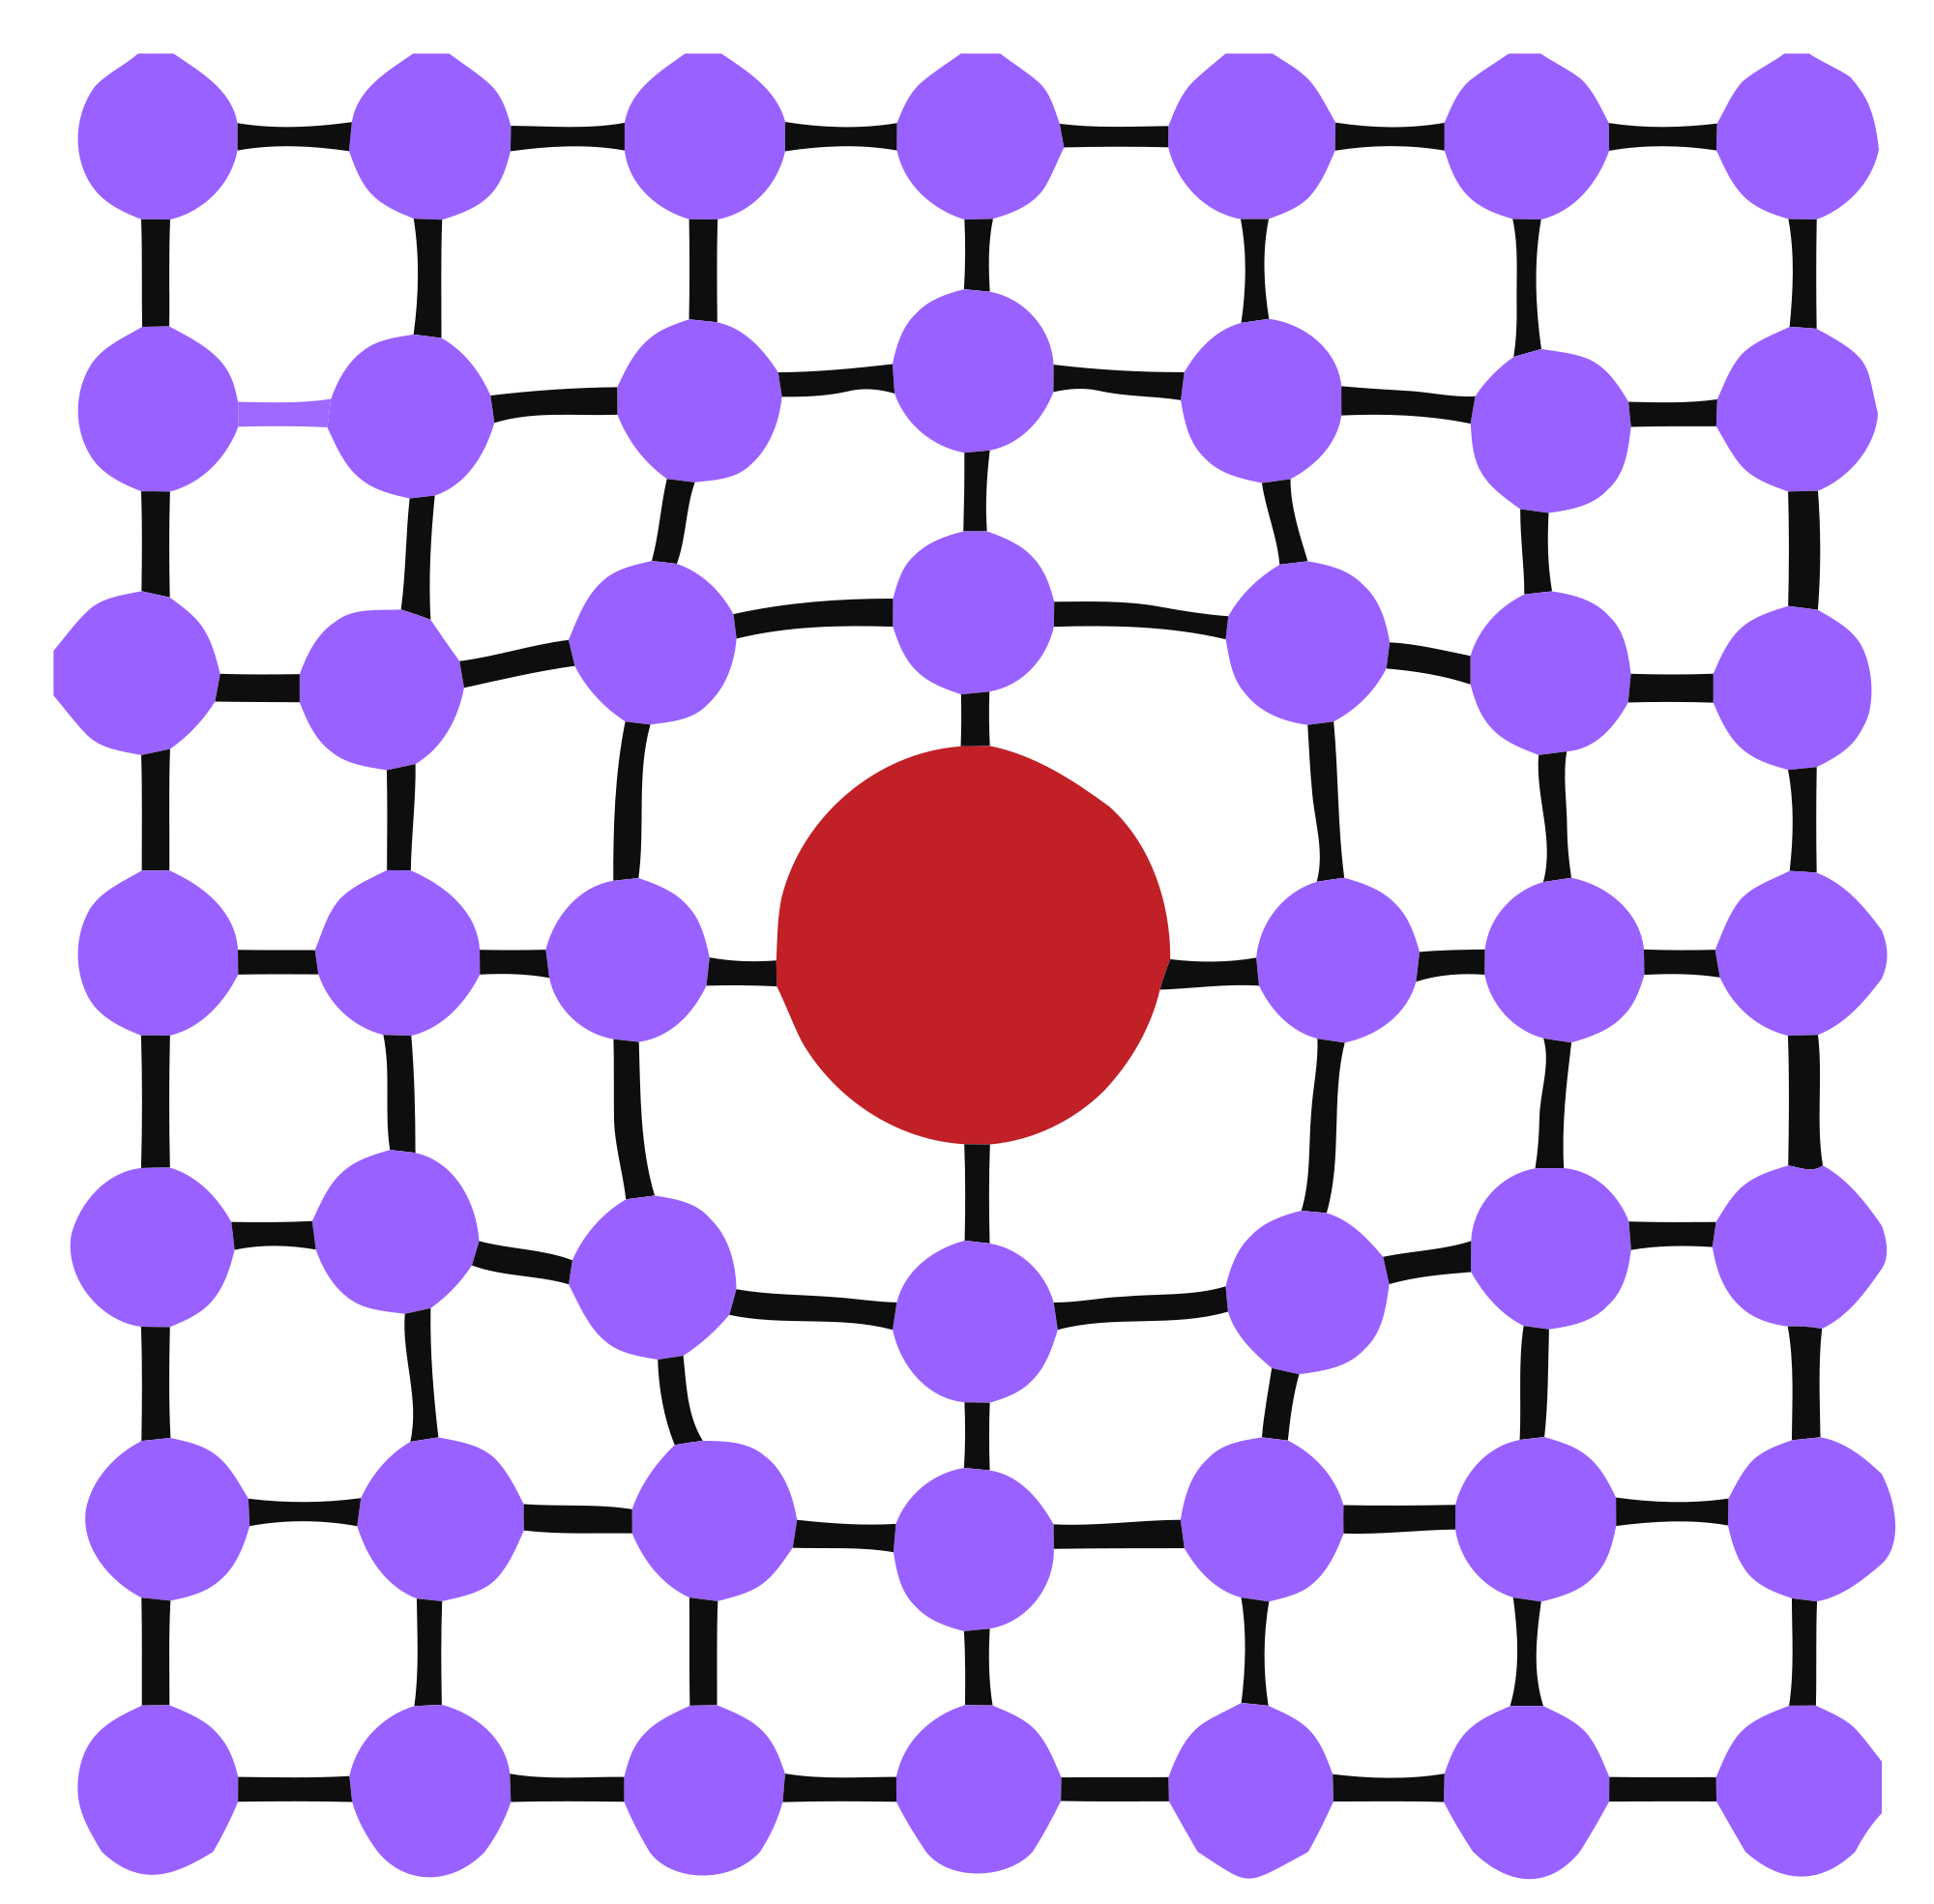
\includegraphics[width=0.19\textwidth]{defect-1.png}\qquad
% 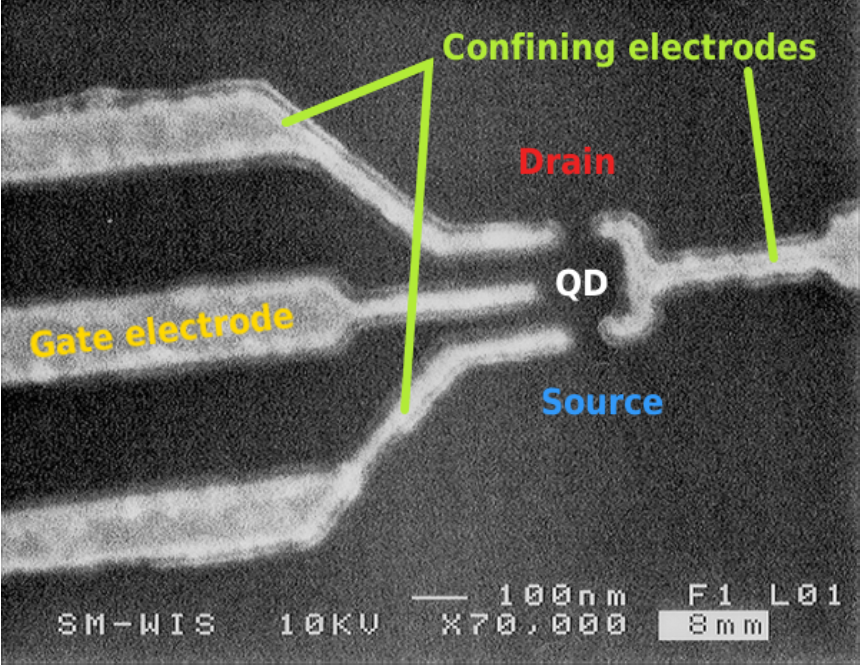
\includegraphics[width=0.24\textwidth]{SET.png}\qquad
% 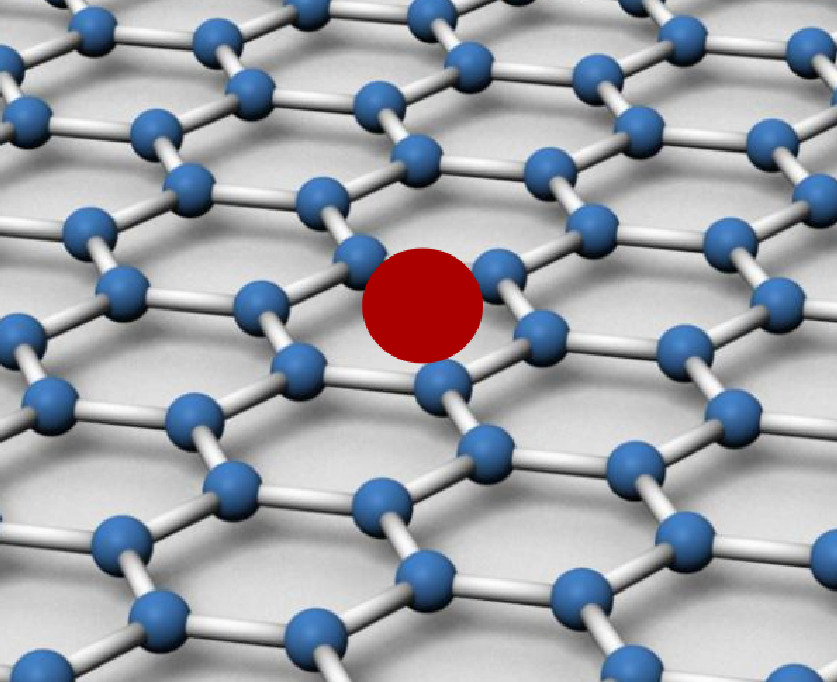
\includegraphics[width=0.23\textwidth]{graphene3.png}
% \end{figure}
% ~~~~~~~~~~~~~~~~3D稀磁合金~~~~~~~~~~~~量子点2DEG~~~~~~~~~~~~2D吸附原子石墨烯
% \end{frame}

\subsection{1.1近藤效应}
\title{铁磁石墨烯中近藤效应的NRG研究\qquad \qquad \qquad \qquad 近藤问题的历史}
\begin{frame}{稀磁合金中的近藤效应}
\begin{minipage}[t]{0.4 \textwidth}
\begin{figure}
\centering
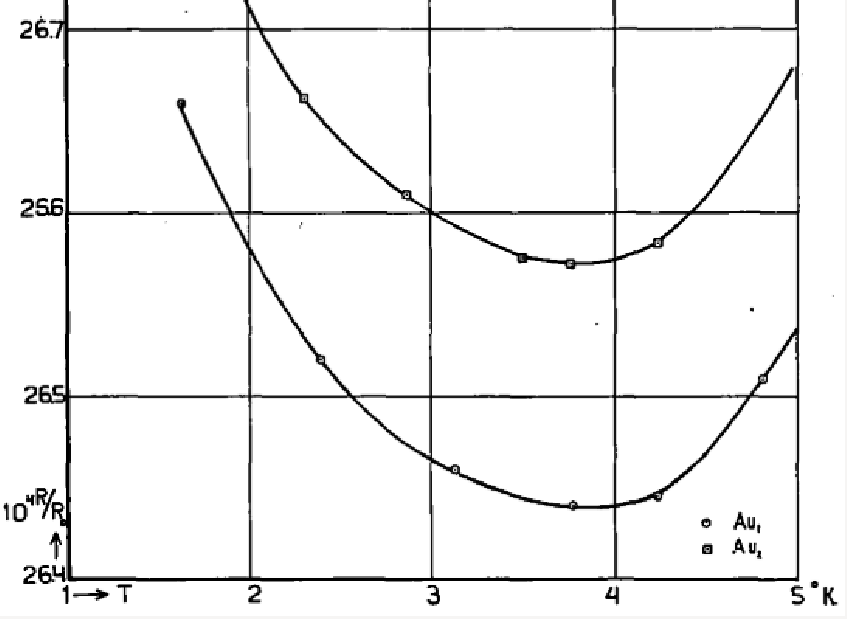
\includegraphics[width=\textwidth]{kondo-deHaas.png}
Physica, 1934, 1(7):1115\\ \ \\
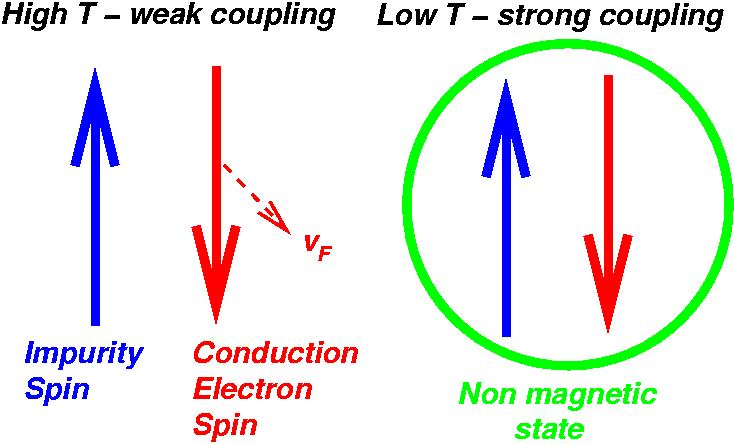
\includegraphics[width=0.9\textwidth]{Kscheme.jpg}
\end{figure}
\end{minipage}%
\begin{minipage}[t]{0.6 \textwidth}
\vspace{0.3cm}
\begin{itemize}
\setlength\itemsep{0.1em}
\item 1934年,de Haas在Fe/Au,低温电阻极小值
% \item 1964年,Sarachik,实验上,电阻反常与局域磁矩形成有关
\item 1964年,Kondo,三阶微扰论,考虑高阶过程,得到电阻的对数贡献,近藤效应
\begin{figure}
\centering
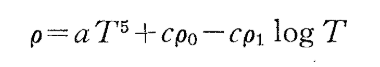
\includegraphics[width=0.6\textwidth]{kondo-resistivity.png}
\end{figure}
\item 特征能量尺度:近藤温度$T_{k}$
% \item 1975年,Wilson数值重整化群(NRG)
\item 物理机制:当$T<T_{k}$时,传导电子屏蔽了杂质磁矩,共同形成了近藤单态,改变系统输运性质
\end{itemize}
\ \\ \ \\
出现近藤效应的条件:
\begin{itemize}
\item[1.] 杂质形成局域磁矩:系统参数处于近藤区
\item[2.] 费米面上有足够的电子来屏蔽局域磁矩:$\rho(E_{F})\neq 0$
\item[3.] 高阶的量子效应占主导:$T<T_{k}$
\end{itemize}
\end{minipage}
\end{frame}

% \begin{frame}{量子点中的近藤效应}
% \begin{minipage}[t]{0.5 \textwidth}
% \begin{figure}
% 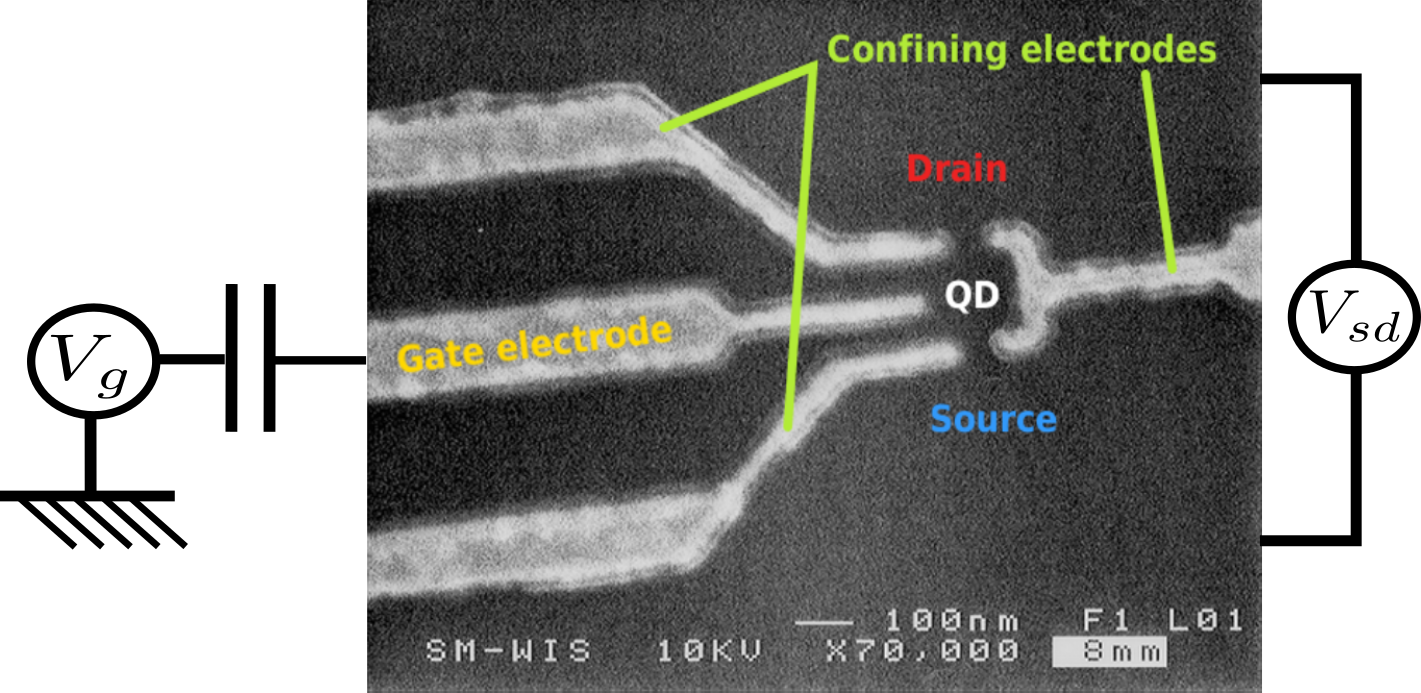
\includegraphics[width=0.49\textwidth,height=0.3\textwidth]{QD.png}
% 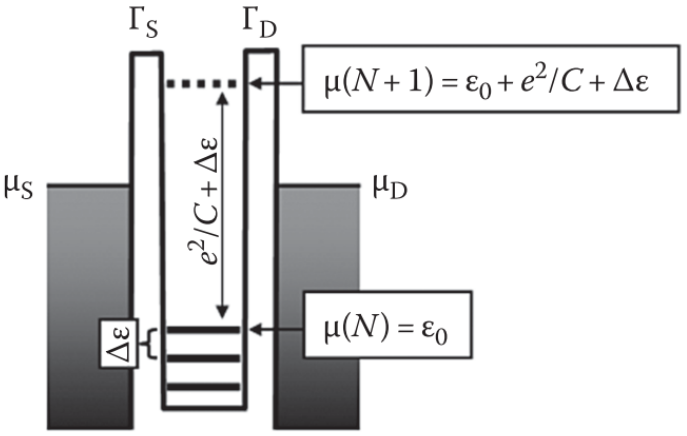
\includegraphics[width=0.49\textwidth,height=0.3\textwidth]{QD1.png}\\
% SET(最早的量子点)~~~~~~能量空间示意图~~~~~~\\
% 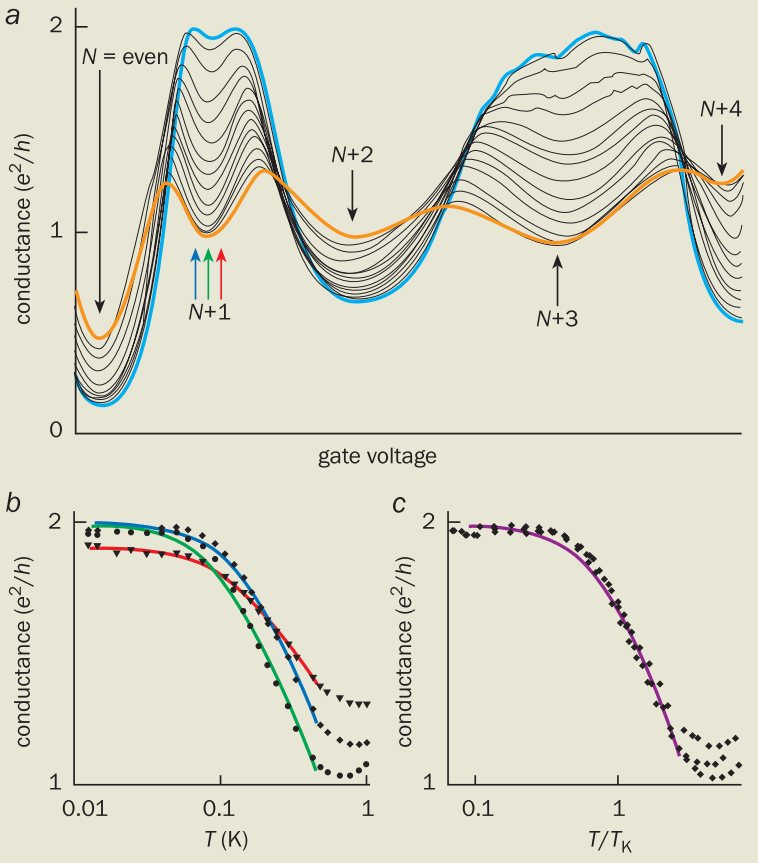
\includegraphics[width=\textwidth,height=4.8cm]{condct.png}\\
% Physical World \textbf{14}, 33
% \end{figure}
% \end{minipage}%
% \begin{minipage}[t]{0.5 \textwidth}
% 单杂质Anderson模型:\\
% \footnotesize
% $H= \sum_{k, \sigma} \varepsilon_{k \sigma} c_{k \sigma}^{\dagger} c_{k \sigma} + \sum_{\sigma}\left(\epsilon_{d} d_{\sigma}^{\dagger} d_{\sigma}+\frac{U}{2} n_{\sigma}^{\dagger} n_{\overline{\sigma}}\right)\\
% + \sum_{k, \sigma} \frac{V}{\sqrt{2 N}}\left(c_{k \sigma}^{\dagger} d_{\sigma} + \mathrm{H.c.}\right).$
% \small
% \begin{itemize}
% \setlength\itemsep{0.4em}
% \item 量子点高度可调控:$T, V_{g}, V_{sd}, \Gamma_{s},\Gamma_{d}$
% \item 1998年,Goldhaber-Gordon, Nature \textbf{391}, 156
% \item 温度降低时,近藤谷内电导$G-V_{g}$增强(形成局域磁矩),谷外电导减小(没有形成局域磁矩)
% \item 随着温度降低,电导增强呈对数(与金属中近藤效应相同)
% \item 不同$V_{g}$处的电导随温度变化曲线可以用近藤温度$T_{k}$标度
% \item 出现近藤效应的条件:
% \begin{itemize}
% \item[1.] 杂质形成局域磁矩:系统参数处于近藤区
% \item[2.] 费米面上有足够的电子来屏蔽局域磁矩:$\rho(E_{F})\neq 0$
% \item[3.] 高阶的量子效应占主导:$T<T_{k}$
% \end{itemize}
% \end{itemize}
% \end{minipage}
% \end{frame}

\subsection{1.2量子点中的近藤效应}
% \title{铁磁石墨烯中近藤效应的NRG研究\qquad \qquad \qquad 那么,什么是近藤效应?}
% \begin{frame}{量子点中的近藤效应}
% \begin{figure}
% 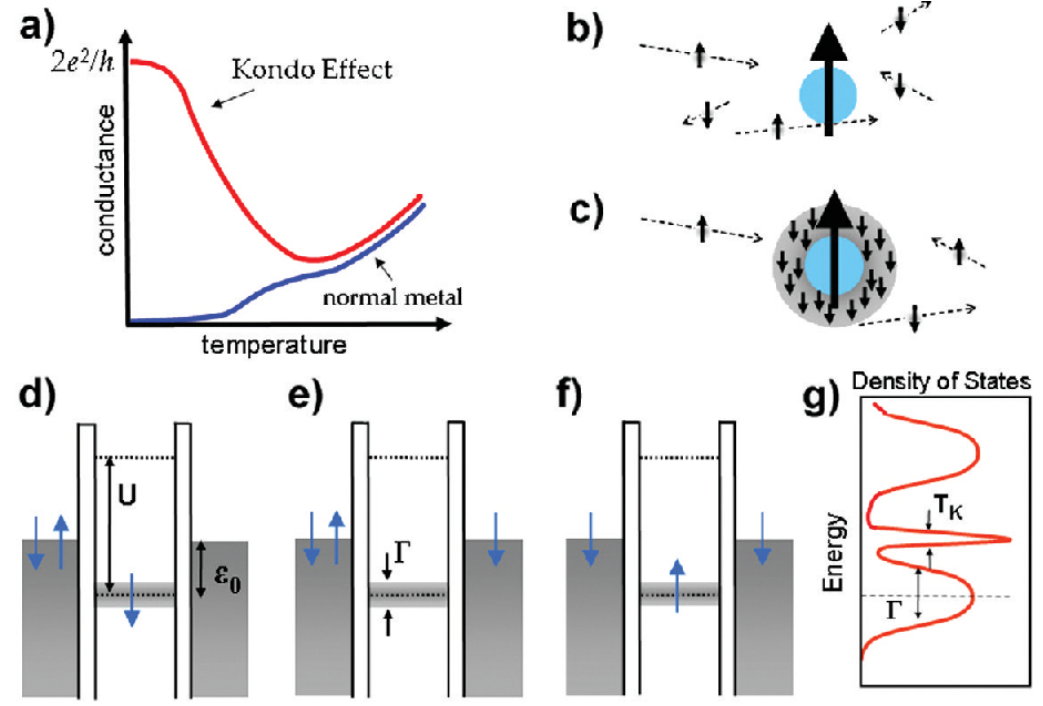
\includegraphics[width=0.85\textwidth]{kondo_effect.png}
% \end{figure}
% \end{frame}

\title{铁磁石墨烯中近藤效应的NRG研究\qquad \qquad \qquad \qquad 背景}
\begin{frame}{量子点中电极铁磁性对近藤物理影响}
\begin{minipage}[t]{0.55 \textwidth}
单杂质Anderson模型+NRG\\
金属电极的杂化函数为常数:
\[
\begin{array}{l}{\Gamma_{\uparrow}(\omega)=\Gamma_{\uparrow}} \\ {\Gamma_{\downarrow}(\omega)=\Gamma_{\downarrow}}\end{array}
\]
自旋极化参数$P$标志铁磁电极中铁磁性的强弱:
\[
\begin{aligned} P \equiv &\left(\Gamma_{\uparrow}-\Gamma_{\downarrow}\right) /\left(\Gamma_{\uparrow}+\Gamma_{\downarrow}\right) \\ & \Gamma_{\uparrow(\downarrow)}=\frac{1}{2} \Gamma(1 \pm P) \end{aligned}
\]
\begin{itemize}
\item p-h对称,铁磁性$P$不抑制近藤共振(abc)
\item p-h非对称,铁磁性$P$抑制近藤共振(def)
\item 近藤峰劈裂,峰高度下降、宽度变宽、位置变远
\end{itemize}
\vspace{0.3cm}
\center{铁磁性的引入,抑制了已经形成的近藤共振!}
\end{minipage}%
\begin{minipage}[t]{0.5 \textwidth}
\vspace{-0.3cm}
\begin{figure}
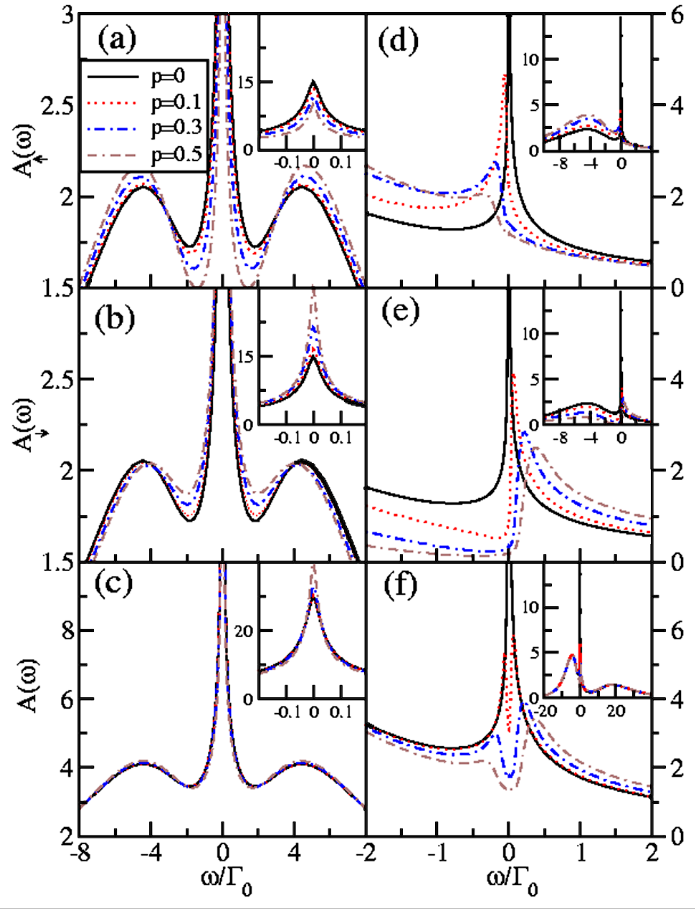
\includegraphics[width=0.9\textwidth]{Aw-P.png}
% 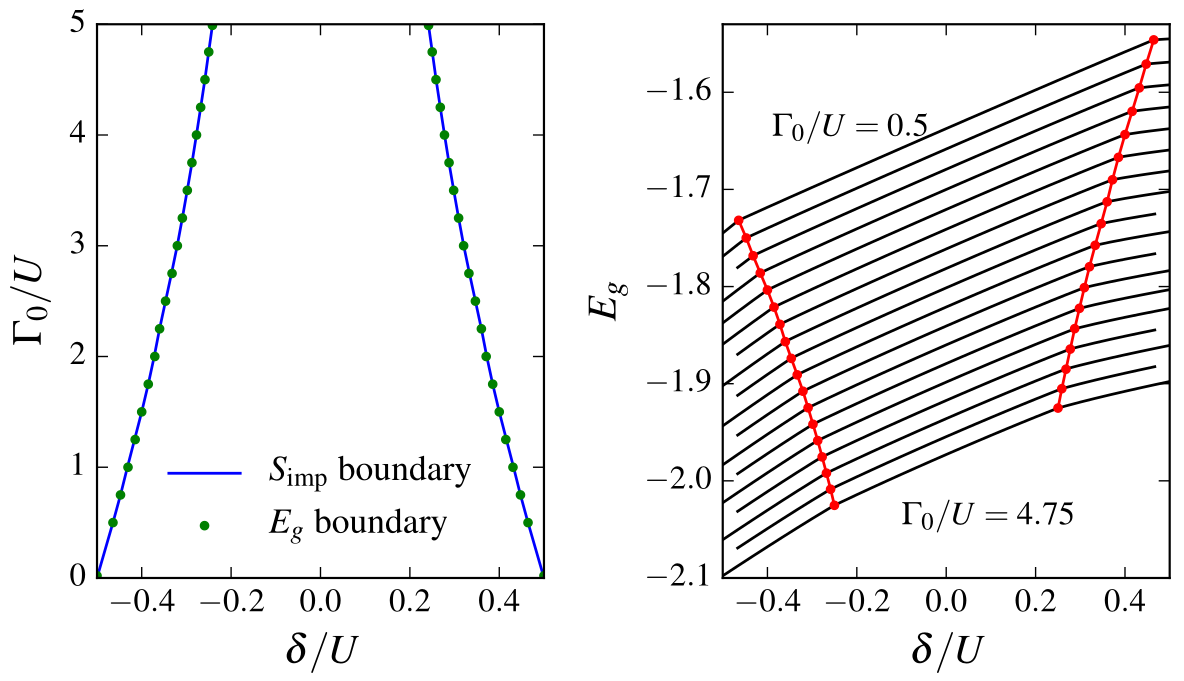
\includegraphics[width=0.9\textwidth,height=0.7\textwidth]{Eg.png}
\end{figure}
\vspace{-0.4cm}
\center{PRL \textbf{92}, 056601}
% PRL \textbf{92}, 056601
\end{minipage}
\end{frame}
\subsection{1.3石墨烯中的近藤效应}
% \title{铁磁石墨烯中近藤效应的NRG研究\qquad \qquad \qquad \qquad 背景}
% \begin{frame}{量子点中外磁场对铁磁近藤的补偿}
% \vspace{0.5cm}
% \begin{minipage}[t]{0.55 \textwidth}
% 电极铁磁性$P$,补偿磁场$B$:
% \[P\neq 0, B\neq 0\]
% 作用在杂质能级上的Zeeman场:
% \begin{equation}\nonumber
% H_{\mathrm{Zeeman}}=-g \mu_{B} B S_{z}
% \end{equation}
% 定义临界补偿磁场$B_{c}$:\\
% \vspace{-0.5cm}
% \center{磁场补偿掉电极铁磁性时,$n_{\uparrow}=n_{\downarrow}$}
% \vspace{0.2cm}
% \begin{itemize}
% \item 铁磁性$P$导致近藤峰劈裂
% \item 磁场$B$可以抵消铁磁性$P$导致的近藤劈裂
% \item $B=B_{c}$时,近藤峰高度回复到幺正极限
% \end{itemize}
% \vspace{0.6cm}
% 劈裂的近藤峰 $\rightarrow$ 近藤峰 $\rightarrow$ 劈裂的近藤峰
% \end{minipage}%
% \begin{minipage}[t]{0.5 \textwidth}
% \begin{figure}
% 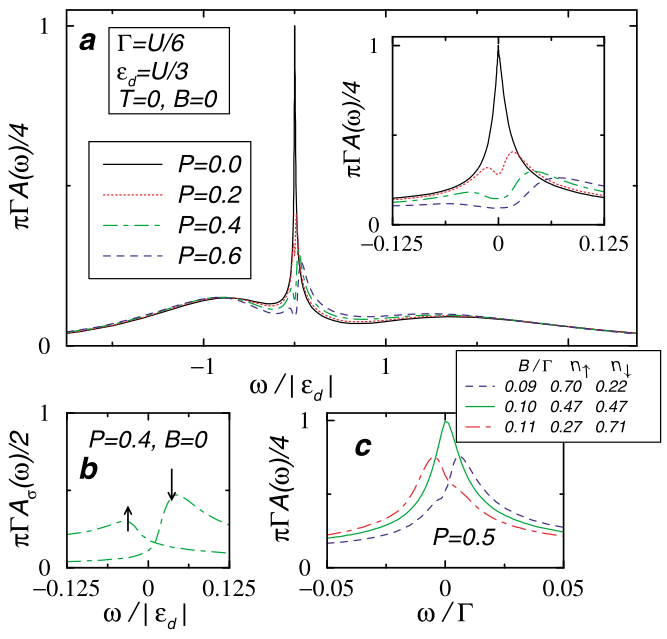
\includegraphics[width=0.91\textwidth]{split-P-compensation.png}
% \end{figure}
% \center{PRL \textbf{91}, 247202}
% \end{minipage}
% \end{frame}
\title{铁磁石墨烯中近藤效应的NRG研究\qquad \qquad \qquad \qquad 背景}
\begin{frame}{量子点中外磁场对铁磁近藤的补偿}
% \vspace{1.6cm}
\begin{minipage}[t]{0.55 \textwidth}
电极铁磁性$P\neq 0$,补偿磁场$B\neq 0$\\
作用在杂质能级上的Zeeman场:
\begin{equation}\nonumber
H_{\mathrm{Zeeman}}=-g \mu_{B} B S_{z}
\end{equation}
定义临界补偿磁场$B_{c}$:\\
\vspace{-0.5cm}
\center{磁场补偿掉电极铁磁性时,$n_{\uparrow}=n_{\downarrow}$}
% \vspace{0.2cm}
\begin{itemize}
\item 补偿磁场$B_{c}$随铁磁性$P$的变化曲线对粒子空穴的依赖
\item $B=B_{c}$时,近藤峰高度回复到幺正极限
\item 被补偿后的近藤峰高度相近,但宽度随$P$增大而减小
\item 近藤温度$T_{k}$随$P$增大而减小
\item 可以用$T_{k}(P=0)$标度
\end{itemize}
\end{minipage}%
\begin{minipage}[t]{0.45 \textwidth}
% \vspace{-1.5cm}
\begin{figure}
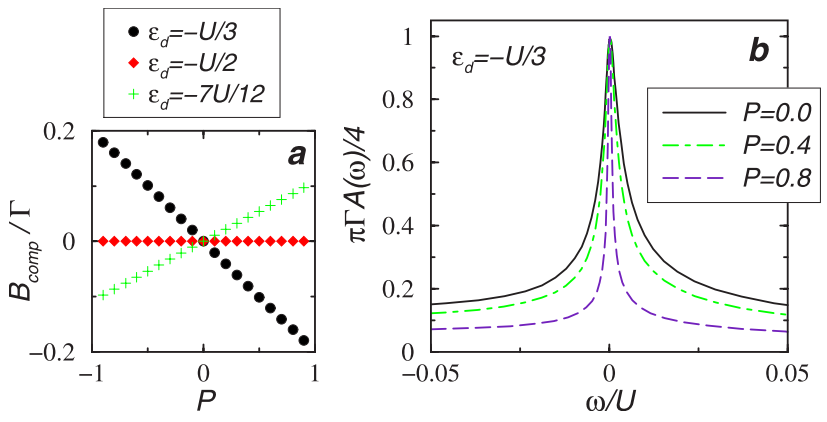
\includegraphics[width=\textwidth]{Aw-P-Bc.png}
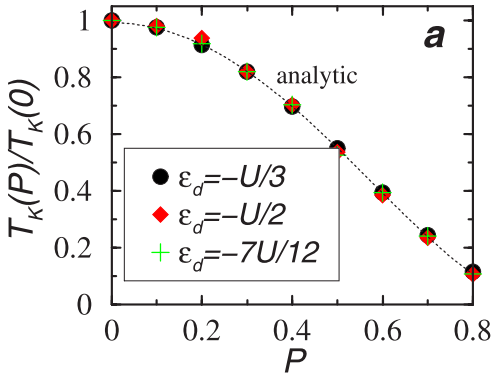
\includegraphics[width=0.6\textwidth]{Tk-P.png}
\end{figure}
\center{PRB \textbf{76}, 045321}
\end{minipage}
\vspace{0.4cm}
\center{磁场抵消了铁磁电极中的铁磁性,完全回复到了纯的近藤共振态!}
\end{frame}
\title{铁磁石墨烯中近藤效应的NRG研究\qquad \qquad \qquad 石墨烯的奇特性质}
\begin{frame}{石墨烯的性质}
\begin{figure}
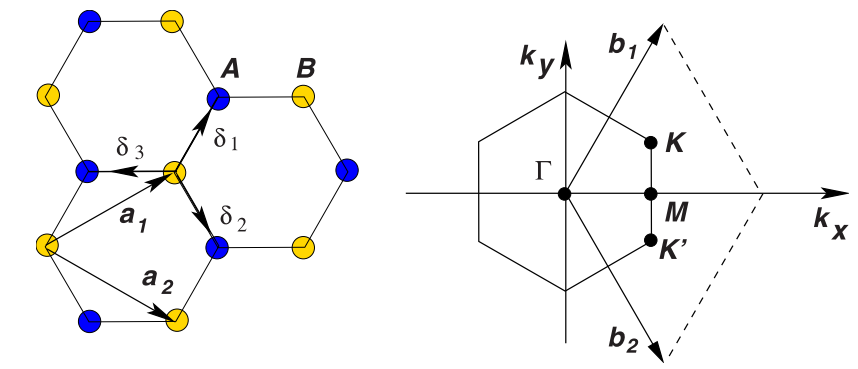
\includegraphics[width=0.47\textwidth]{graphene2.png}
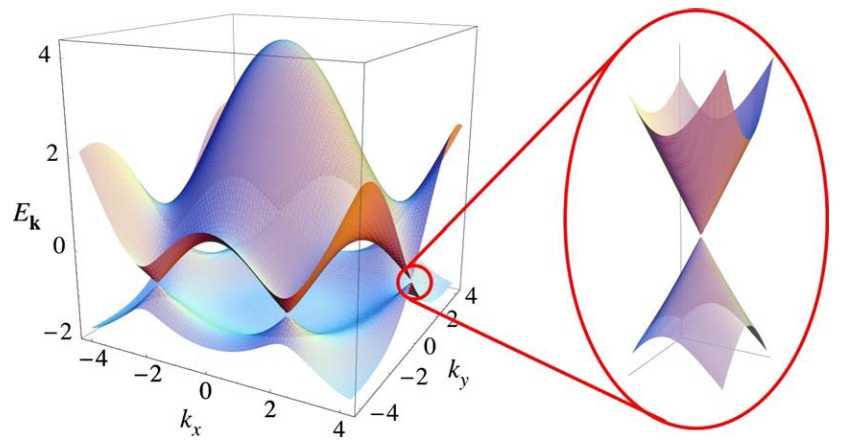
\includegraphics[width=0.4\textwidth]{graphene1.png}
\end{figure}
紧束缚近似下最近邻耦合:
$H_{\mathrm{g}}=\varepsilon_{0}\sum_{i, \sigma}\left(a_{i \sigma}^{\dagger} a_{i \sigma}+b_{i \sigma}^{\dagger} b_{i \sigma}\right) - t \sum_{\langle i j\rangle, \sigma} \left(a_{i \sigma}^{\dagger} b_{j \sigma}+\mathrm{H.c.}\right)$\\
在狄拉克$K$点附近: \qquad \qquad \qquad \quad $\varepsilon_{\pm}(k)\sim \pm v_f |k|$\\
态密度:\qquad \qquad \qquad \qquad \qquad \qquad  $\rho(\varepsilon)=\frac{2 A_{c}}{\pi} \frac{|\varepsilon|}{v_{F}^{2}}\propto |\varepsilon|$
\begin{figure}
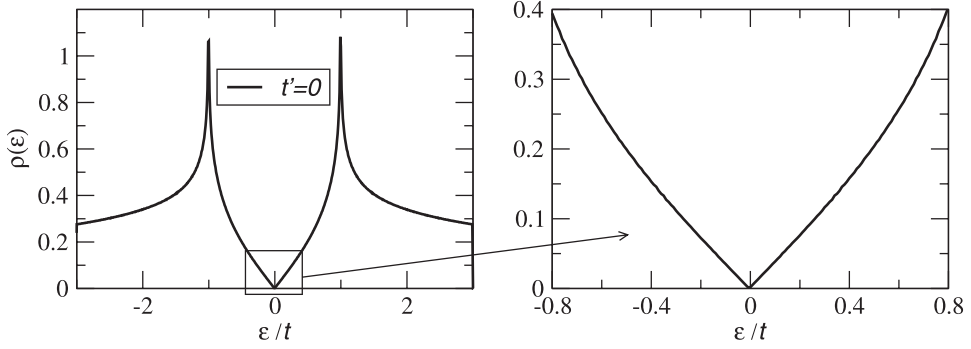
\includegraphics[width=0.6\textwidth]{graphene-dos.png}
\end{figure}
\end{frame}
\subsection{1.4研究动机}
\title{铁磁石墨烯中近藤效应的NRG研究\qquad \qquad \qquad \qquad 研究动机}
\begin{frame}{研究动机}
\begin{figure}
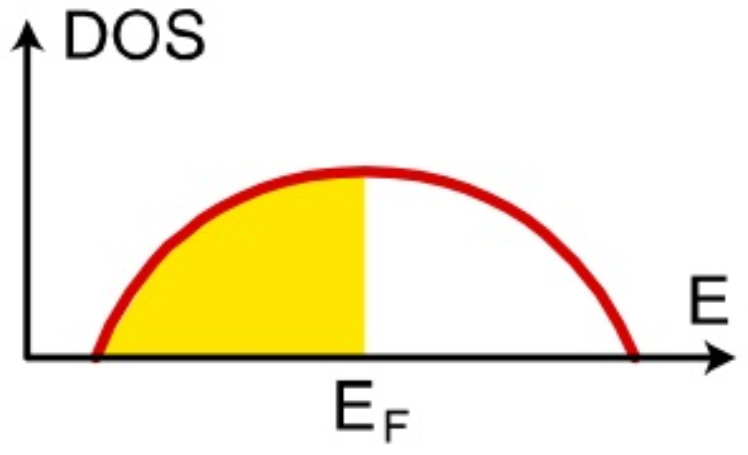
\includegraphics[width=0.3\textwidth,height=0.25\textwidth]{metal-dos.png}
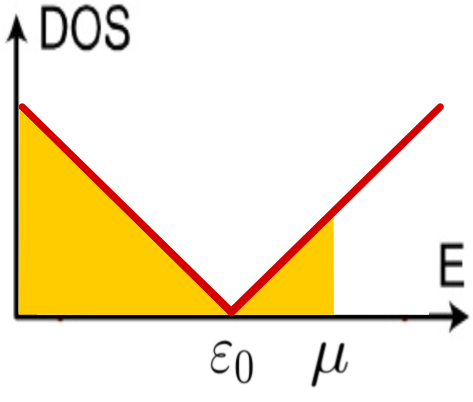
\includegraphics[width=0.3\textwidth,height=0.25\textwidth]{gated-dos.png}
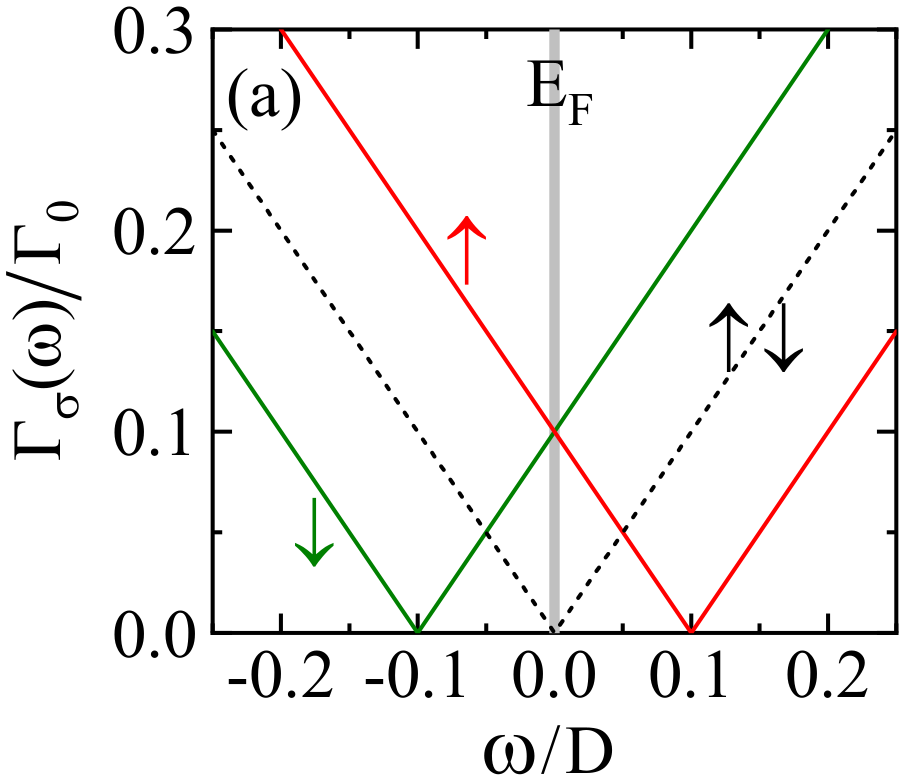
\includegraphics[width=0.3\textwidth,height=0.25\textwidth]{hyb1.png}
\end{figure}
~~~~~~~~~~$\rho(\omega)=\rm{const}$~~~~~~~~~~~~~~~~~~$\rho(\omega)=|\omega+\mu|$~~~~~~~~~~~~~~~~~~~~~~~$\rho_{\sigma}(\omega)=|\omega-\sigma h|$\\
~~~~~~稀磁合金、量子点系统~~~~~~~~~~受门电压调节的石墨烯~~~~~~~~~~~~~~~引入铁磁性$h$\\ \ \\
\begin{itemize}
\setlength\itemsep{0.4em}
\item[1.] 在石墨烯中引入铁磁性$h$,能否产生近藤共振?
\item[2.] 如果能,会对近藤共振有什么影响?抑制?增强?
\item[3.] 门电压调节化学势$\mu$与铁磁性$h$的共同作用对近藤物理的影响?
\item[4.] 外磁场$B$能不能调节近藤共振?
\end{itemize}
\end{frame}
% \title{铁磁石墨烯中近藤效应的NRG研究\qquad \qquad \qquad \qquad 门电压调控}
% \begin{frame}{石墨烯中的近藤效应}
% \normalsize
% 在石墨烯中实现局域磁矩:吸附磁性原子、点缺陷
% \begin{itemize}
% \item 电中性石墨烯($\mu=0$)中的近藤效应:$r=1$赝能隙近藤问题, $\rho(\omega)\propto |\omega|^{r}$
% \begin{itemize}
% \setlength\itemsep{0.4em}
% \item[1.] 粒子空穴对称时,不能出现近藤效应
% \item[2.] 偏离粒子空空对称点,且耦合强度大于临界值时,会才能出现近藤效应
% \item[3.] 实验证据:Co/Graphene,Nano Letters, 2014, 14(7):4011–4015; 点缺陷石墨烯,Nature Communications, 2018, 9(1):2349.
% \end{itemize}
% \item 对石墨烯注入电子或空穴($\mu\neq 0$),将费米面移开狄拉克点,$\rho(\omega)\propto |\omega+\mu|$。
% \begin{itemize}
% \setlength\itemsep{0.4em}
% \item[1.] $\rho(E_{F})\neq 0$,可以产生近藤屏蔽
% \item[2.] 化学势$\mu$可以用来调节打开或关闭近藤效应
% \item[3.] $\mu$具体对近藤物理的影响,如$T_{k}(\mu), \Gamma_{c}(\mu), n_{\rm{imp}}(\mu)$
% \end{itemize}
% \end{itemize}
% \begin{figure}
% 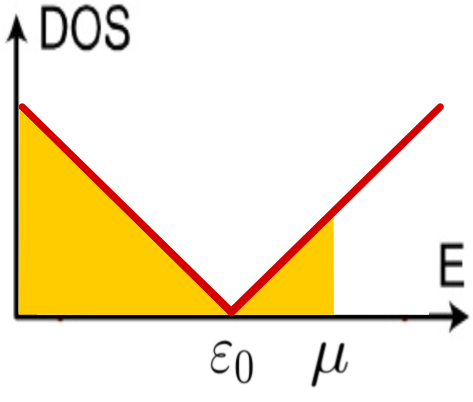
\includegraphics[width=0.3\textwidth]{gated-dos.png}
% 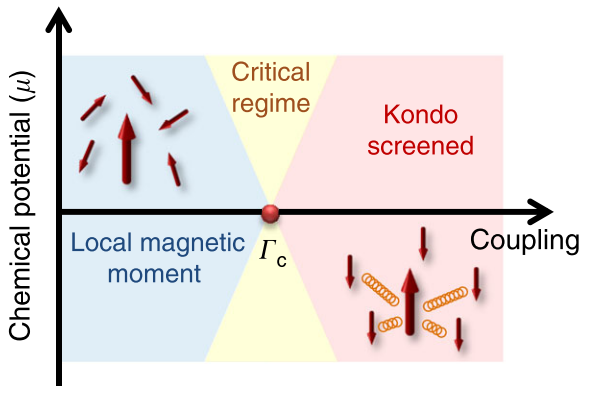
\includegraphics[width=0.35\textwidth,height=0.25\textwidth]{phasediagram.png}
% 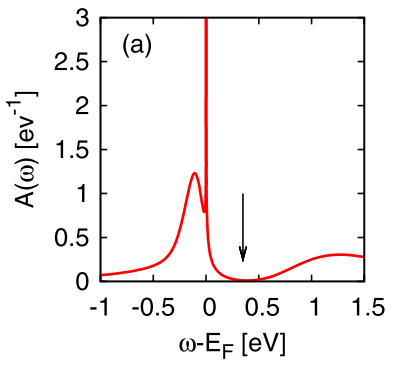
\includegraphics[width=0.3\textwidth,height=0.25\textwidth]{dos-gated.png}
% \end{figure}
% \end{frame}
\subsection{1.5研究方法: 全密度矩阵数值重整化群 (FDM-NRG)}
\title{铁磁石墨烯中近藤效应的NRG研究\qquad \qquad \qquad \qquad NRG}
\begin{frame}{传统数值重整化群 (Wilson's NRG)}
\begin{itemize}
\setlength\itemsep{0.4em}
\item[1.] 1975 K. G. Wilson为解决近藤问题设计。重整化群操作的数值化:
\[
H_{N+1}=R\left(H_{N}\right)
\]
\[
 H_{N+1}= \sqrt{\Lambda} H_{N}+\Lambda^{N / 2} \sum_{\sigma} \varepsilon_{N+1} c_{N+1 \sigma}^{\dagger} c_{N+1 \sigma} +\Lambda^{N / 2} \sum_{\sigma} t_{N}\left(c_{N \sigma}^{\dagger} c_{N+1 \sigma}+c_{N+1 \sigma}^{\dagger} c_{N \sigma}\right)
\]
\item[2.] 对数离散化(c)、截断对角化(d),截断机制:保留能量最低的$N_{s}$个态
\item[3.] NRG实现了能量尺度的分离,通过迭代进行截断对角化的方式不断地将高能态舍弃,最终只得到了最低能量尺度的$N_{s}$个态用以计算我们感兴趣的低能物理
\end{itemize}
\begin{figure}
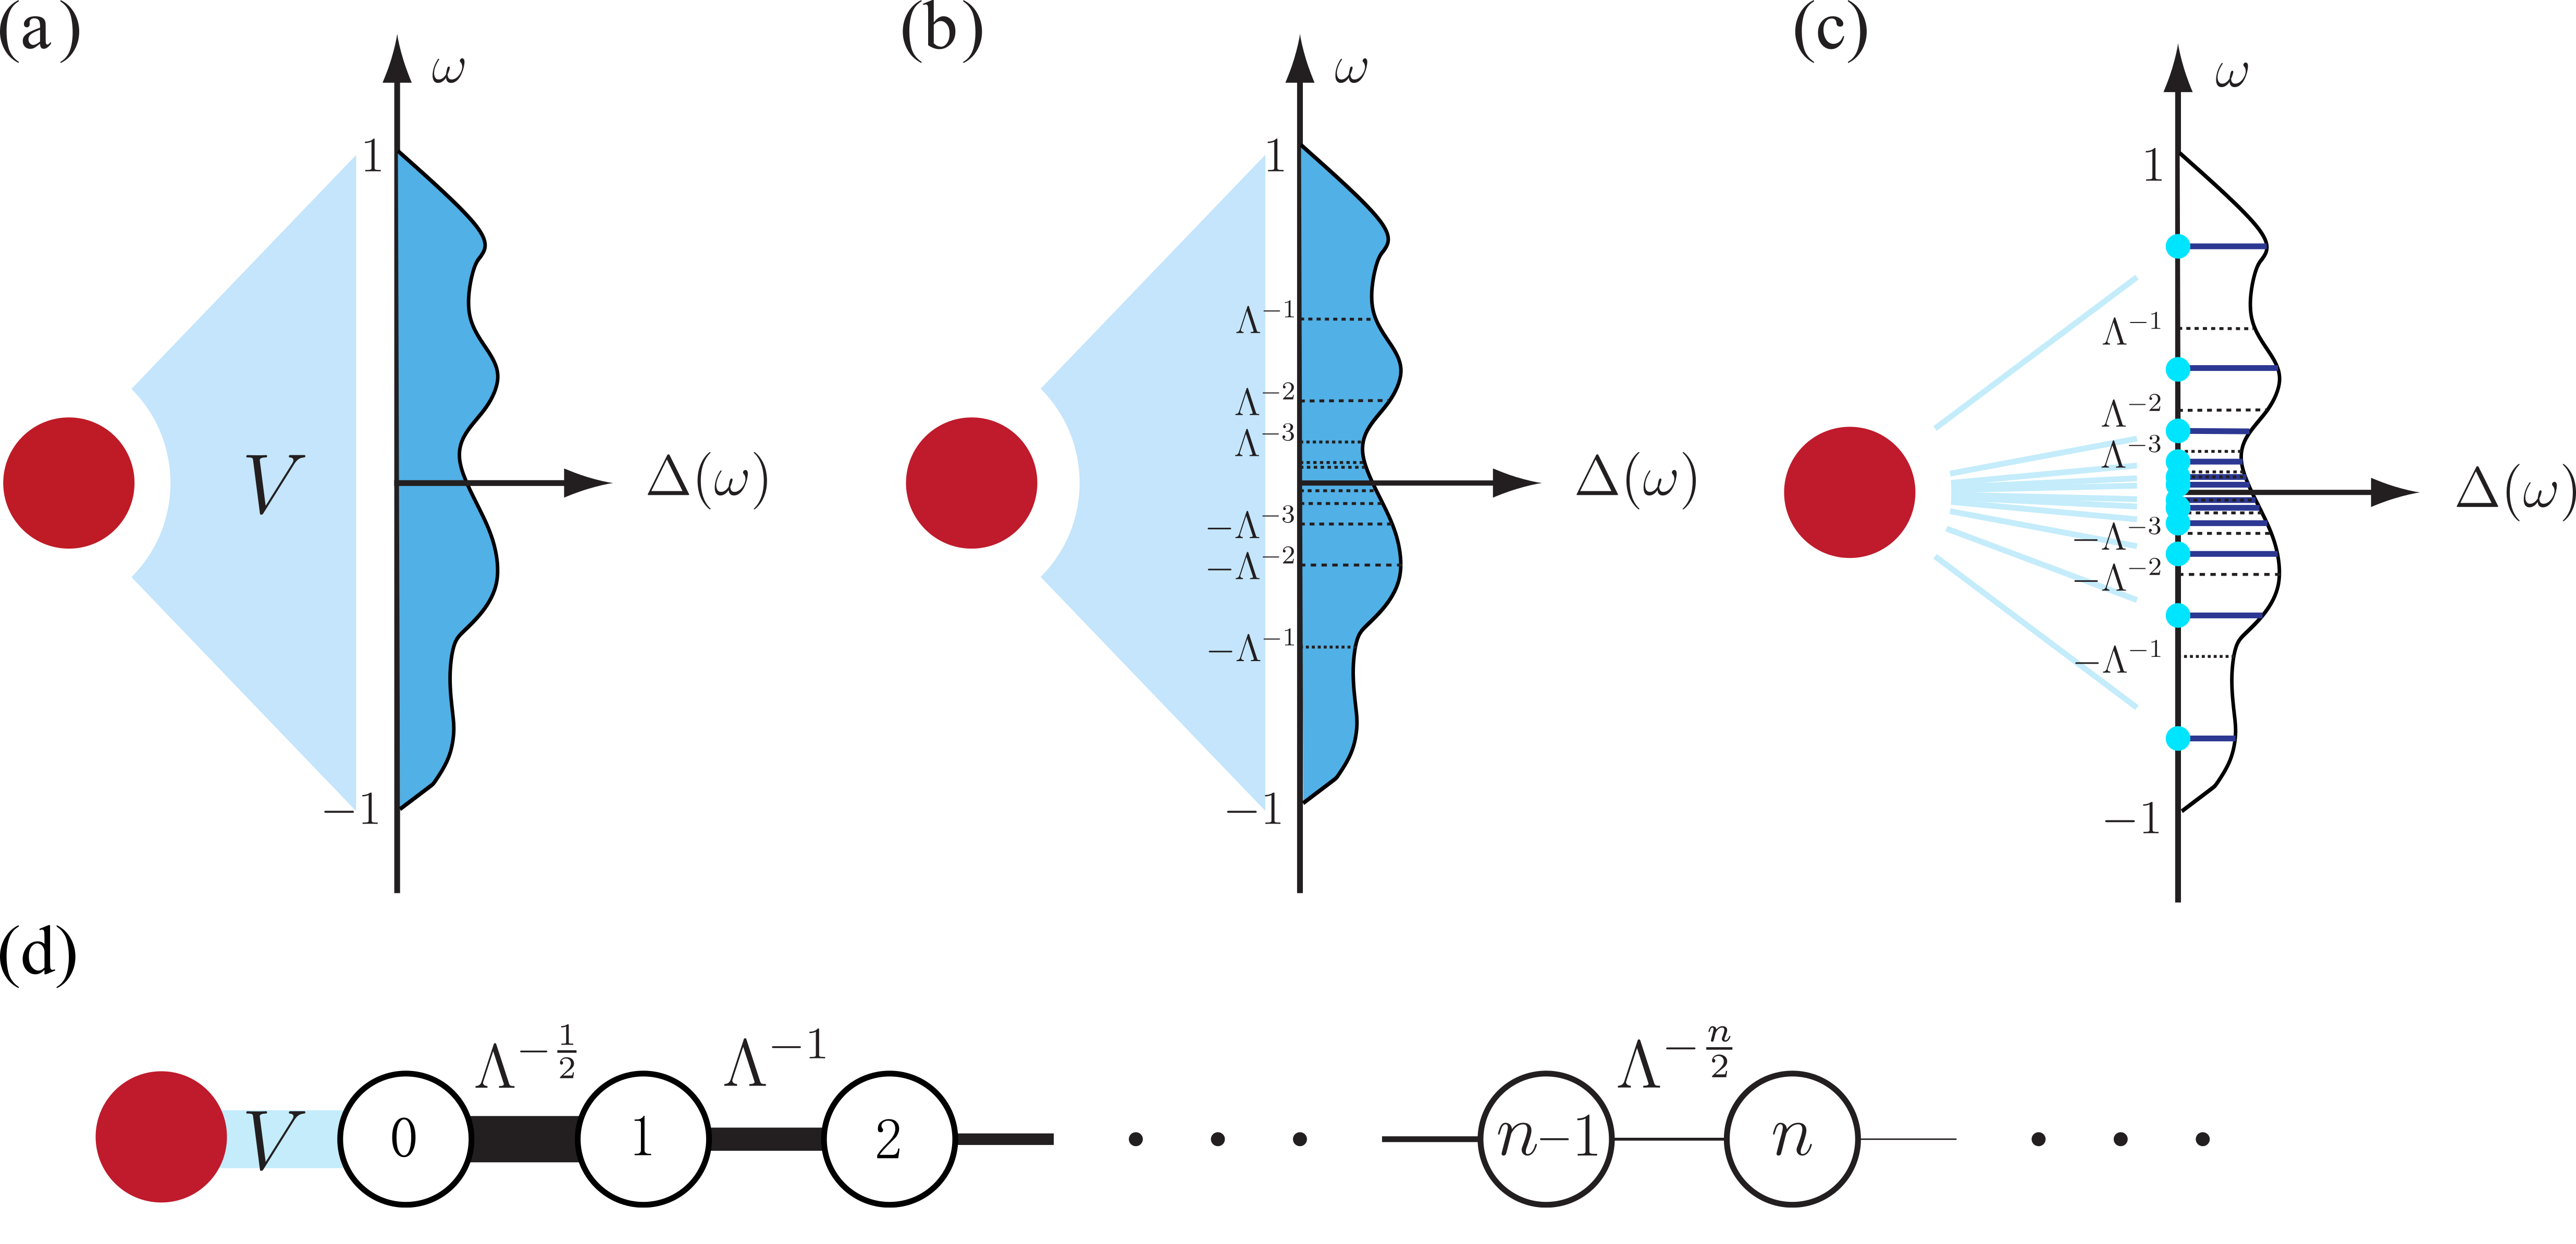
\includegraphics[width=0.7\textwidth,height=0.29\textwidth]{NRGmapping.png}
\end{figure}
\[
|s\rangle_{n}^{\mathrm{X}}=\sum_{s^{\prime} \sigma_{n}}\left[A_{\mathrm{KX}}^{\left[\sigma_{n}\right]}\right]_{s^{\prime} s}\left|s^{\prime}\right\rangle_{n-1}^{\mathrm{K}} \otimes\left|\sigma_{n}\right\rangle , \qquad X=\{\text{保留、舍弃}\}
\]

\end{frame}
\title{铁磁石墨烯中近藤效应的NRG研究\qquad \qquad \qquad \qquad FDM-NRG}
\begin{frame}{全密度矩阵数值重整化群 (FDM-NRG)}
传统NRG的缺陷:
\begin{itemize}
\setlength\itemsep{0.4em}
\item[1.] 只利用了$N_{s}$个态来计算,不完备
\item[2.] 只利用了最后一个能量尺度的态。当考虑多个能量尺度间的跃迁时,结果将产生严重偏差
\end{itemize}
解决方法:将舍弃的态重新考虑进来,即完备的Anders-Schiller基矢。
\begin{figure}
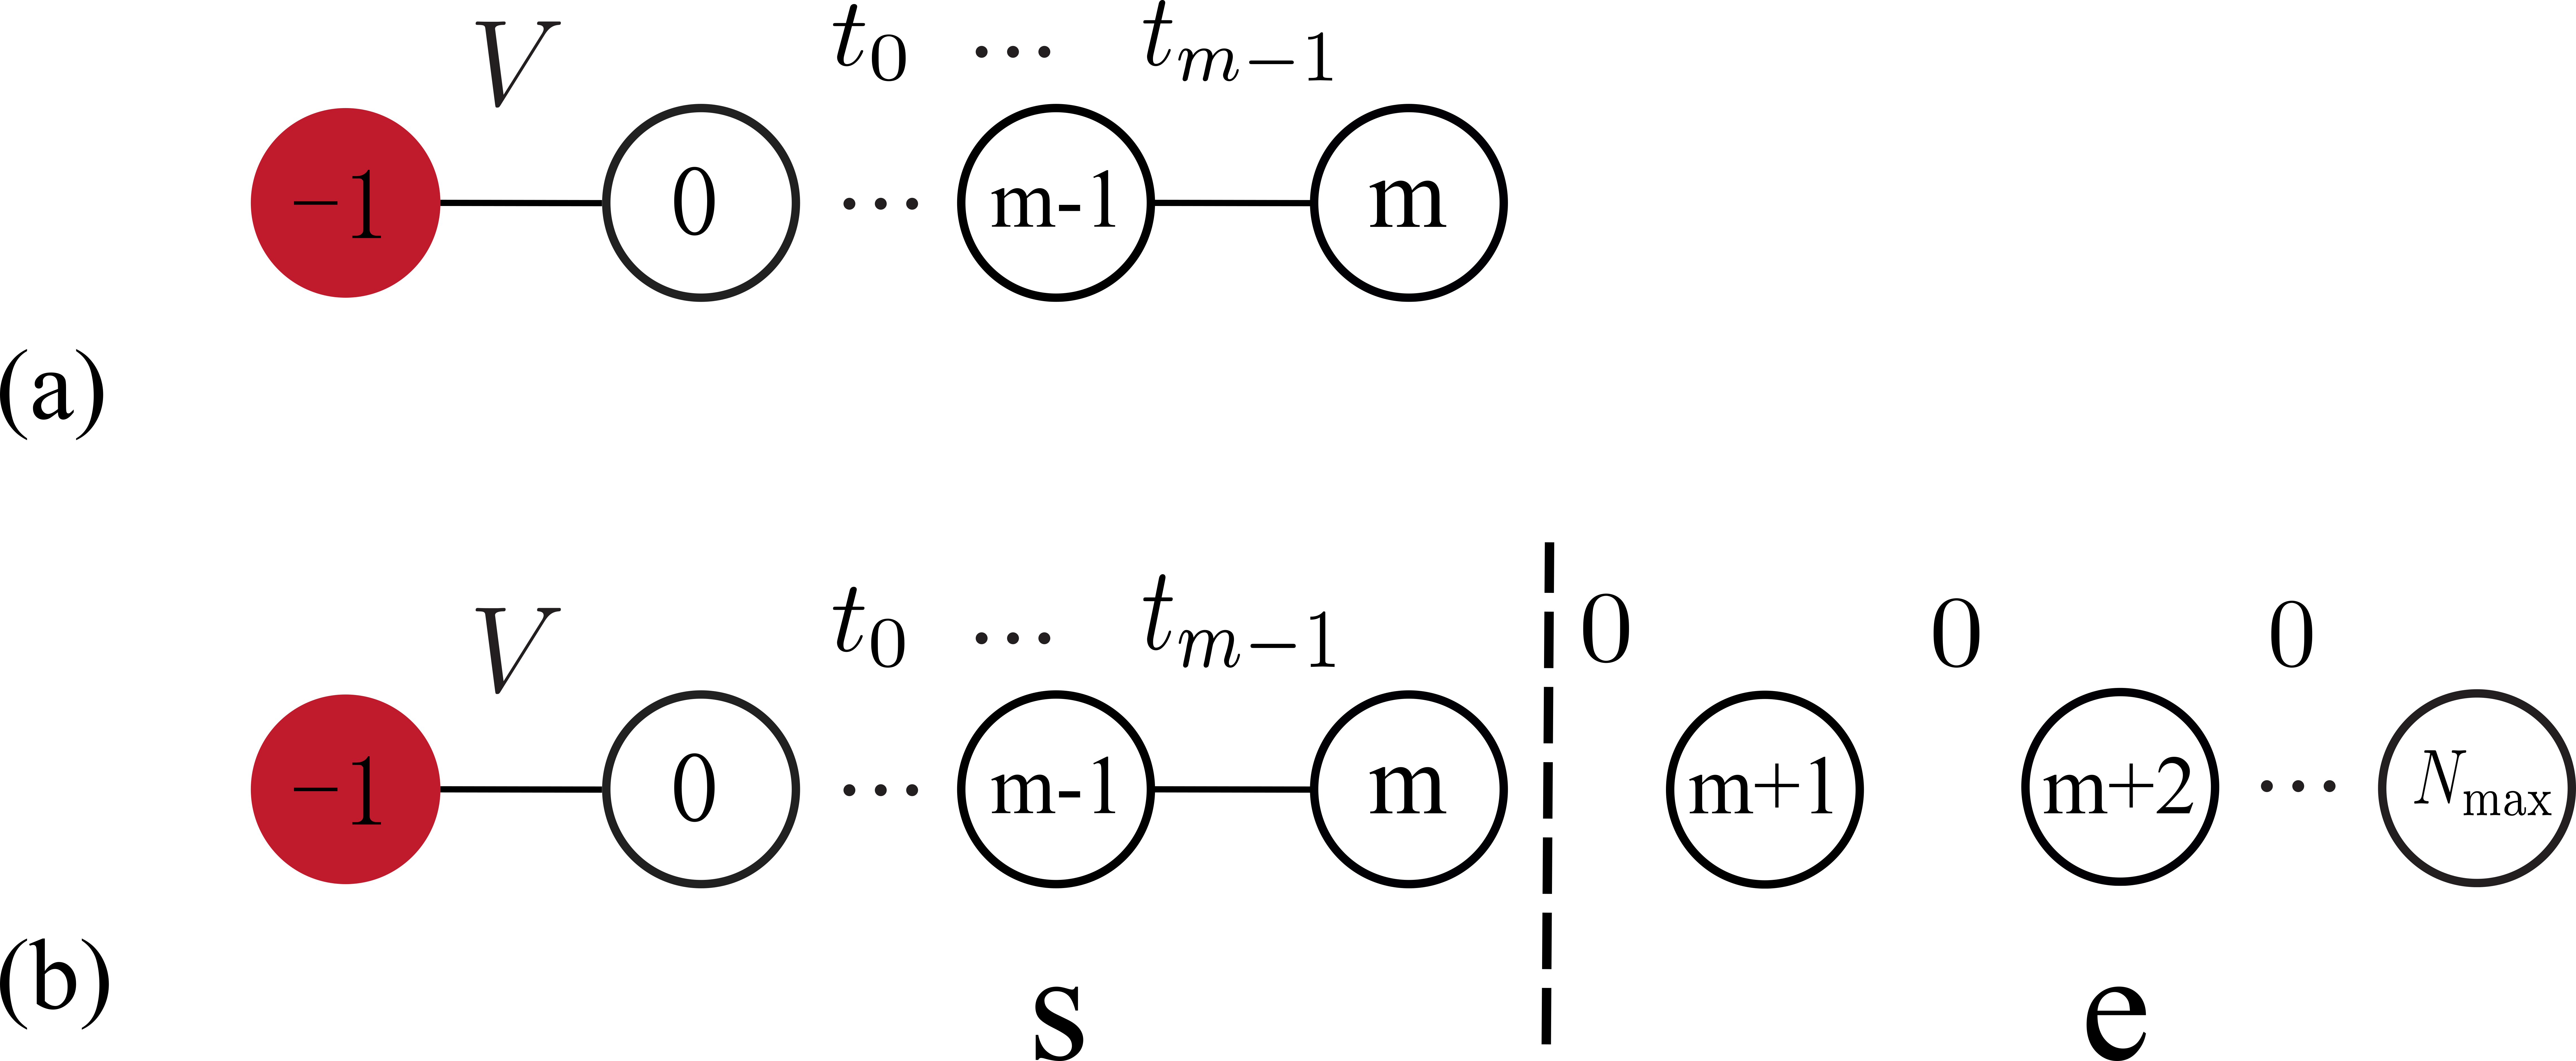
\includegraphics[width=0.5\textwidth]{chain-split.png}
\end{figure}
长点时自动补齐剩下的简并环境态:
\[
|s e\rangle_{N}^{X}=|s\rangle_{N}^{X} \otimes\left|e_{N}\right\rangle
\]
Anders-Schiller基矢:传统NRG中所有舍弃态与简并环境态的直积态的集合,
\begin{equation}\nonumber
\boldsymbol{1}^{(d_{\rm{imp}} d^{N_{\rm{max}}+1})} = \sum_{se}^{X=K,D} \ket{se}_{n_0}^X\hspace{0.8mm}{}_{n_0}^X \hspace{-0.8mm} \bra{se} = \sum_{n\geq n_0}^{N_{\rm{max}}} \sum_{se} \ket{se}_n^D {}_n^{\hspace{0.0mm} D} \bra{se}.
\end{equation}
\end{frame}

\section{2.铁磁石墨烯中的近藤现象}
\subsection{2.1研究系统}
\begin{frame}
\tableofcontents[currentsection] 
\end{frame}

\title{铁磁石墨烯中近藤效应的NRG研究\qquad \qquad \qquad \qquad 模型}
\begin{frame}{研究系统}
\begin{figure}
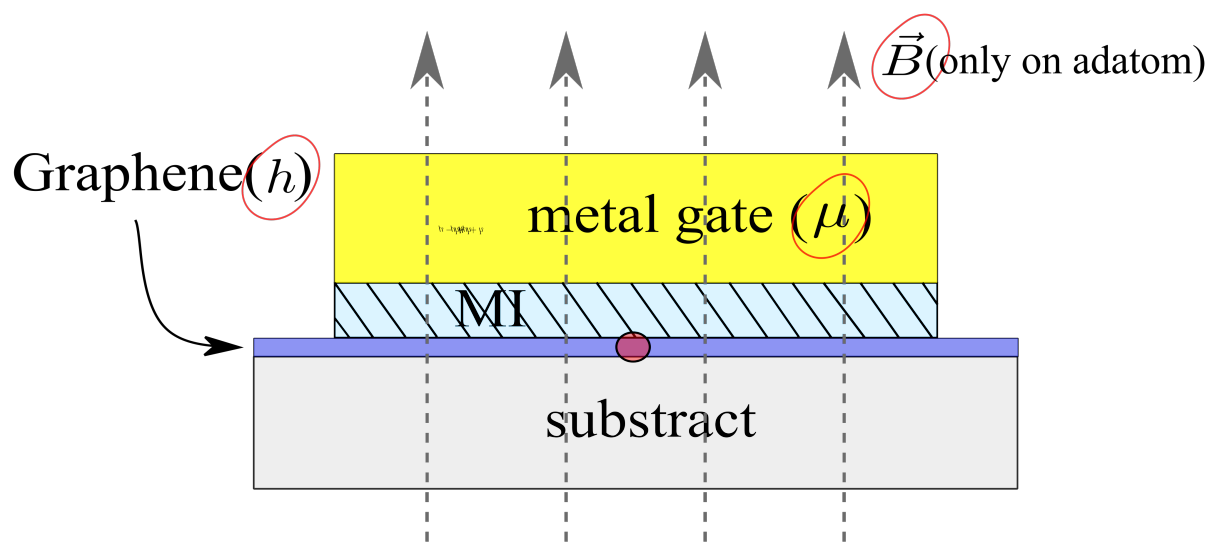
\includegraphics[width=0.45\textwidth]{setup.png}
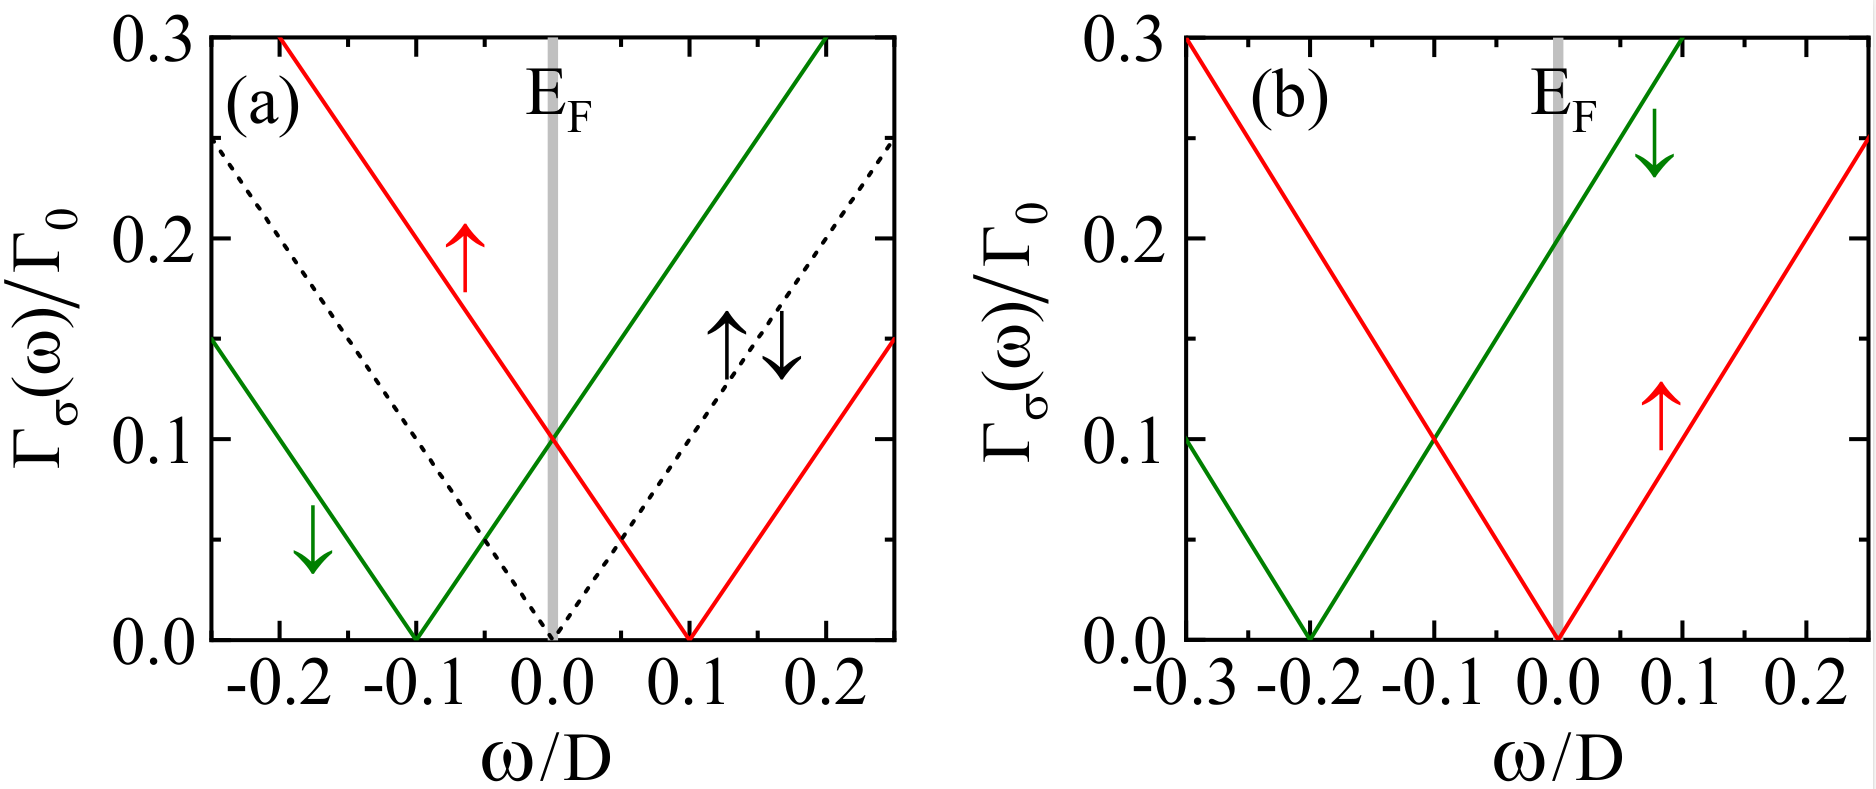
\includegraphics[width=0.5\textwidth]{fig1.png}
\end{figure}
单杂质Anderson模型:
\[
H=\sum_{k, \sigma, \alpha} \varepsilon_{k \sigma \alpha} c_{k \sigma \alpha}^{\dagger} c_{k \sigma \alpha}+\sum_{\sigma}\left(\epsilon_{d \sigma} d_{\sigma}^{\dagger} d_{\sigma}+\frac{U}{2} n_{\sigma}^{\dagger} n_{\bar{\sigma}}\right)+\sum_{k, \sigma, \alpha} \frac{V}{\sqrt{2 N}}\left(c_{k \sigma \alpha}^{\dagger} d_{\sigma}+\mathrm{H.c.}\right)
\]
石墨烯格点信息及调控通过态密度进入杂化函数:
\[
\Gamma_{\sigma}(\omega)=\pi V^{2} \rho_{\sigma}(\omega) = \Gamma_{0}\left|\omega-\varepsilon_{0}+\mu-\sigma h\right|
\]
固定参数:$\qquad \qquad \qquad U=0.2,\delta=0,\Gamma_{0}=0.1,T\ll T_{k}$\\
调控参数:
\begin{itemize}
\setlength\itemsep{0.4em}
\item[1.] 金属门电压调控费米面$\mu$
\item[2.] 通过靠近磁性绝缘体引入石墨烯铁磁性$h$
\item[3.] 置于外磁场$B$中(磁场只引起杂质能级的Zeeman劈裂)
\end{itemize}
\end{frame}

\title{铁磁石墨烯中近藤效应的NRG研究\qquad \qquad 在石墨烯中引入铁磁性会怎么样?铁磁性与近藤共振?}
\begin{frame}{电中性石墨烯的相图}
\begin{minipage}[t]{0.5 \textwidth}
电中性,且未引入铁磁性,无外磁场:
\[\mu=0, h=0, B=0\]
粒子空穴偏移量:
\[\delta=\varepsilon_{d}+U/2\]
其他参数:
\[U=0.2,T=10^{-9},D=1\]
\vspace{-0.45cm}
\begin{itemize}
\item 杂质熵$S_{\rm{imp}}$降为零为相边界确定标准
\item 也可以用基态能量的拐点来确定相边界
\item $S_{\rm{imp}}=0$ 单态,有可能形成近藤屏蔽
\item $S_{\rm{imp}}=1$ 双重态,无近藤屏蔽
\item 杂质谱函数(c)无明显的近藤共振峰\\
($\Gamma_{0} \neq \Gamma_{c}$)
\end{itemize}
\end{minipage}%
\begin{minipage}[t]{0.5 \textwidth}
\begin{figure}
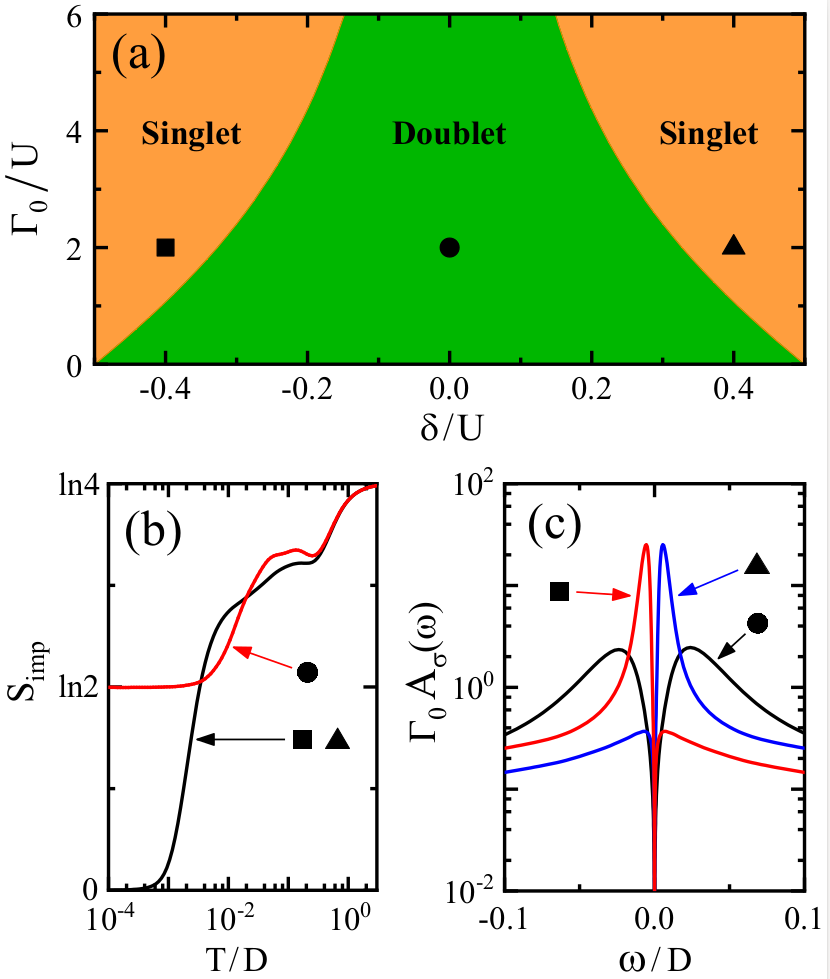
\includegraphics[width=0.9\textwidth]{fig2.png}
\end{figure}
\end{minipage}
\vspace{0.1cm}
\center{之后的讨论均为粒子空穴对称情形(背景介绍除外),$\delta=0$}
\end{frame}
\subsection{2.2铁磁性诱导的近藤屏蔽}
\title{铁磁石墨烯中近藤效应的NRG研究\qquad \qquad \qquad \qquad 近藤肩膀}
\begin{frame}{石墨烯中铁磁性诱导的近藤共振}
\begin{minipage}[t]{0.55 \textwidth}
\begin{minipage}[t]{0.65 \textwidth}
电中性,引入铁磁性,无外磁场:\\
\text{ } \quad $\mu=0, h\neq 0, B=0$
\begin{itemize}
\item $h=0$没有近藤共振
\item $h\neq 0$有肩膀结构
\item 肩膀高度和位置随$h$移动
\end{itemize}
\end{minipage}%
\begin{minipage}[t]{0.45 \textwidth}
\begin{figure}
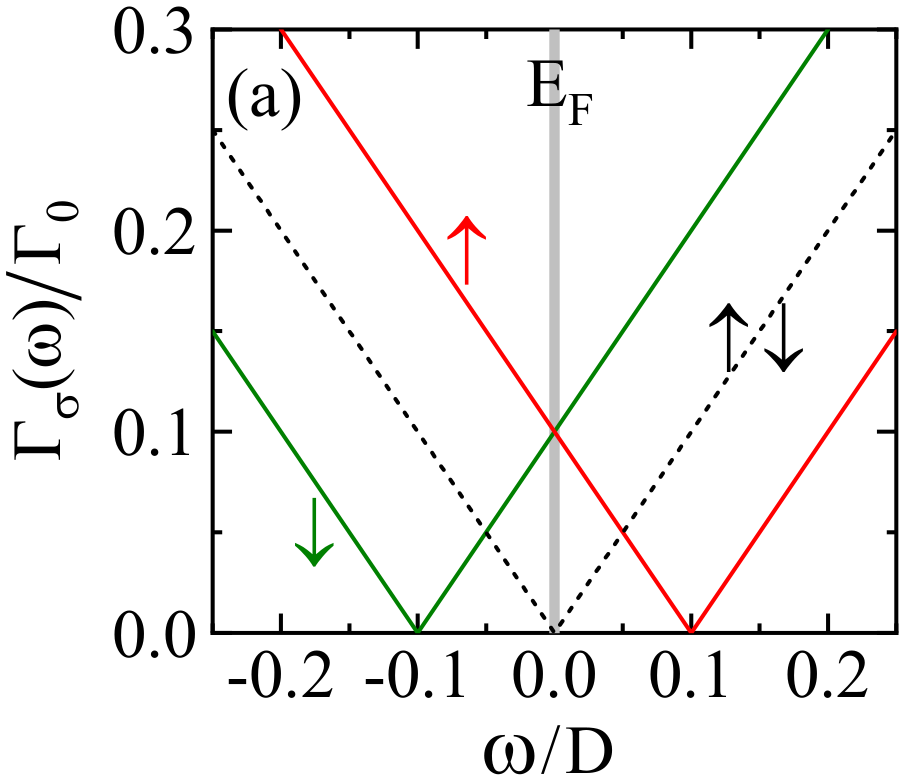
\includegraphics[width=\textwidth]{hyb1.png}
\end{figure}
\end{minipage}
\vspace{-0.4cm}
拟合肩膀位置
\vspace{-0.2cm}
\begin{equation}\nonumber
\begin{aligned} F(\omega) &=F_{1}(\omega)+F_{2}(\omega) \\ F_{1}(\omega)=c_{1} \operatorname{Re} &\left[\left(\frac{i c_{3}}{\omega-c 1+i c 2}\right)^{\frac{1}{2}}\right] \\ F_{2}(\omega) &=c=+c_{5}|\omega| \end{aligned}
\end{equation}
自旋极化的传导电子对杂质能级的有效重整:
\begin{equation}\nonumber
\widetilde{\varepsilon}_{d \sigma}=\varepsilon_{d}-\frac{1}{\pi} \int \mathrm{d} \omega\left\{\frac{\Gamma_{\sigma}(\omega)[1-f(\omega)]}{\omega-\varepsilon_{d}}+\frac{\Gamma_{\bar{\sigma}}(\omega) f(\omega)}{\varepsilon_{d}+U-\omega}\right\}
\end{equation}
近藤劈裂:\qquad \qquad$\Delta=\left|\widetilde{\varepsilon}_{d \uparrow}-\widetilde{\varepsilon}_{d \downarrow}\right|$
\center{肩膀结构来源于近藤共振的贡献!}
\end{minipage}%
\begin{minipage}[t]{0.5 \textwidth}
\vspace{-0.4cm}
\begin{figure}
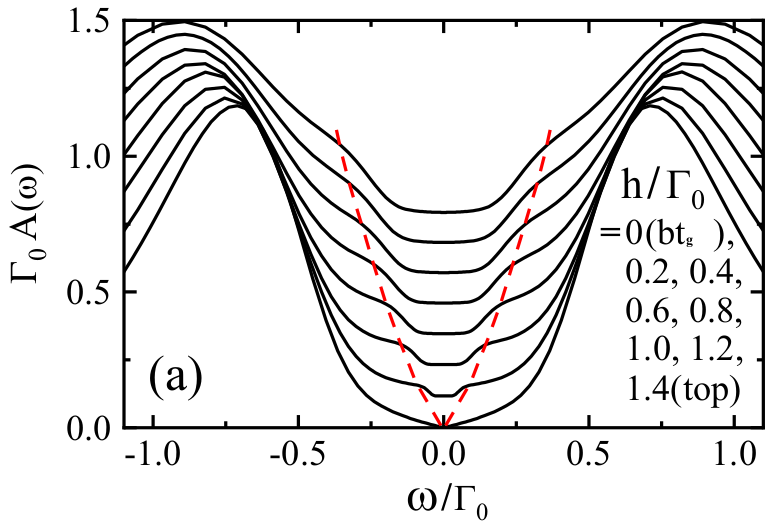
\includegraphics[width=0.75\textwidth]{fig3.png}
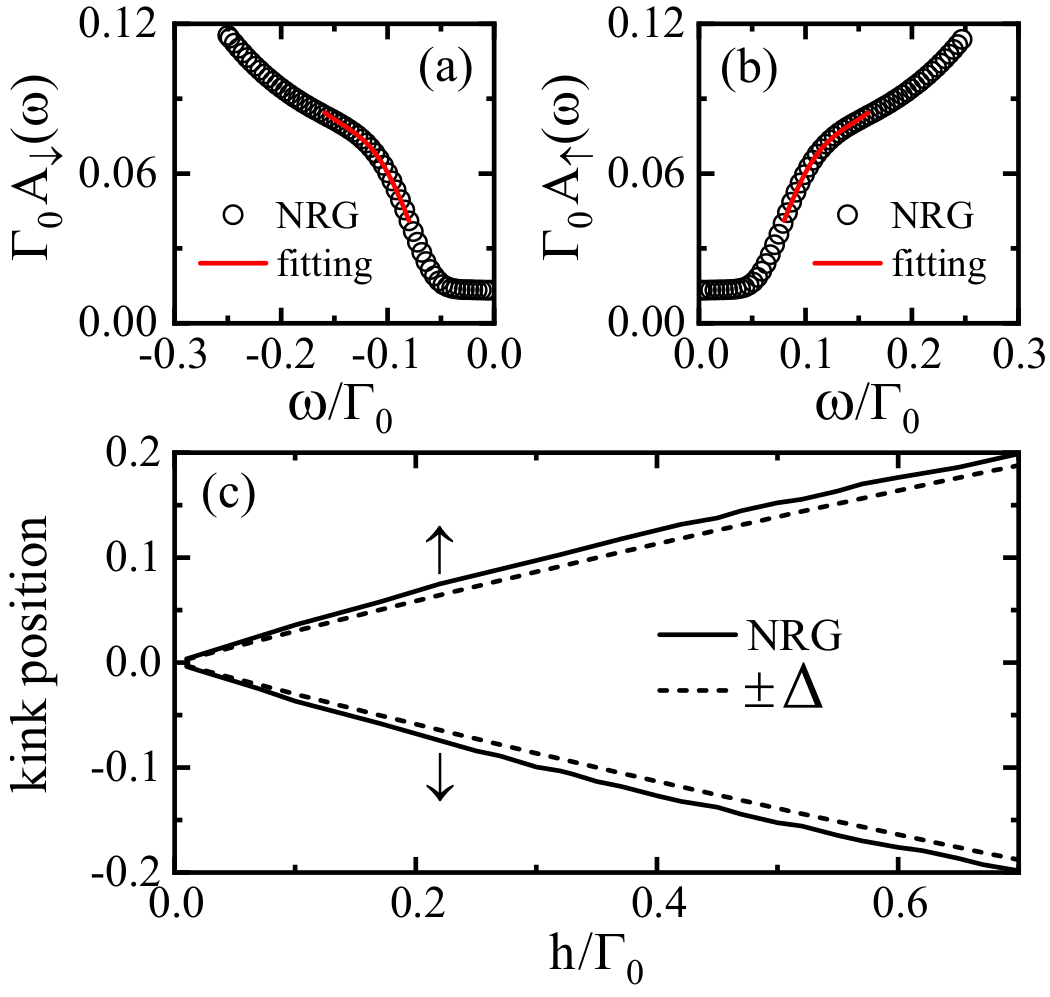
\includegraphics[width=0.75\textwidth]{fig4.png}
\end{figure}
\vspace{-0.4cm}
\center{铁磁性诱导出了石墨烯中的近藤共振!}
\end{minipage}
\end{frame}
\title{铁磁石墨烯中近藤效应的NRG研究\qquad \qquad \qquad \qquad 磁场调控的近藤肩膀}
\begin{frame}{铁磁石墨烯中的近藤补偿效应}
\vspace{0.5cm}
\begin{minipage}[t]{0.55 \textwidth}
石墨烯铁磁性$h$,补偿磁场$B$:
\[\mu=0, h/\Gamma_{0}= 0.5, B\neq 0\]
作用在杂质能级上的Zeeman场:
\begin{equation}\nonumber
H_{\mathrm{Zeeman}}=-g \mu_{B} B S_{z}
\end{equation}
定义补偿磁场$B_{c}$:\\
\vspace{-0.5cm}
\center{磁场补偿掉电极铁磁性时,$n_{\uparrow}=n_{\downarrow}$}
\vspace{0.2cm}
\begin{itemize}
\item 近藤肩膀 $\rightarrow$ 劈裂的近藤峰 \rotatebox[origin=c]{270}{$\Rsh$} \\
\hfill{近藤峰($B_{c}$) \hspace{1cm}}.\\
近藤肩膀 $\leftarrow$ 劈裂的近藤峰 \rotatebox[origin=c]{180}{$\Rsh$}
\item 不能完全看成是磁场抵消了铁磁性(在引入铁磁性$h$和磁场$B$前没有近藤共振)
\item 杂质占据数是过渡行为,没有相变
\end{itemize}
\end{minipage}%
\begin{minipage}[t]{0.55 \textwidth}
\begin{figure}
\hspace{-1.2cm}
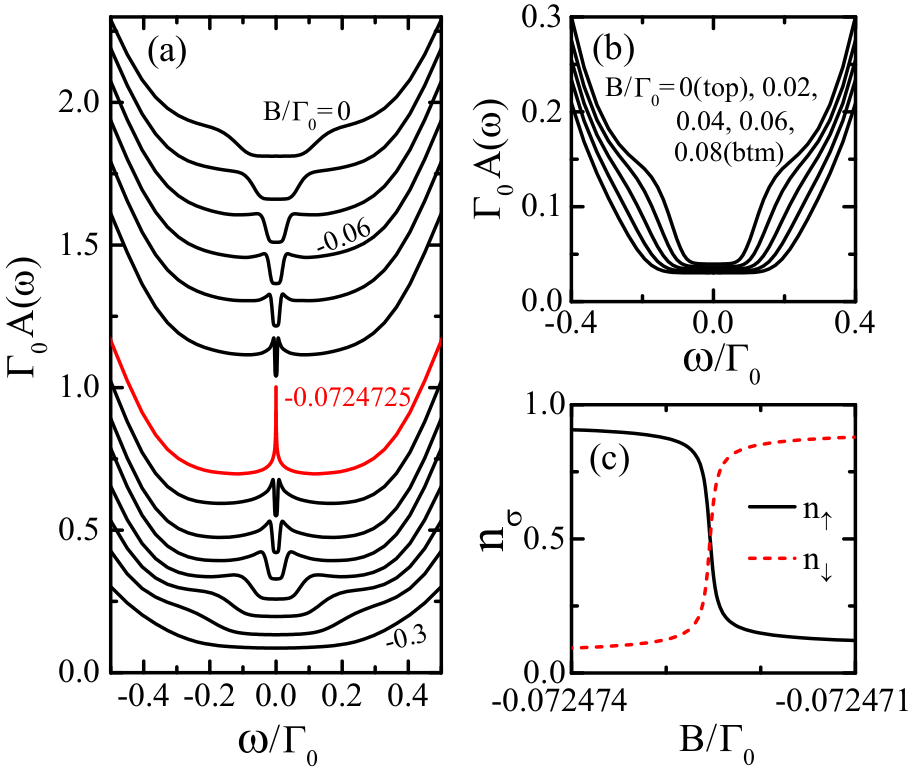
\includegraphics[width=0.9\textwidth]{fig5.png}
\end{figure}
\end{minipage}
\vspace{0.12cm}
\center{自旋极化与近藤共振共存$\underleftrightarrow{\qquad B\qquad}$常规的近藤共振态}
\end{frame}

\title{铁磁石墨烯中近藤效应的NRG研究\qquad \qquad \qquad \qquad 磁场调控的近藤肩膀}
\begin{frame}{补偿点$B_{c}(h)$的性质}
\vspace{0.5cm}
\begin{minipage}[t]{0.55 \textwidth}
\[\mu=0, h\neq 0, B=B_{c}(h)\]
\begin{itemize}
\setlength\itemsep{0.5em}
\item 近藤劈裂$\Delta=\left|\widetilde{\varepsilon}_{d \uparrow}-\widetilde{\varepsilon}_{d \downarrow}\right|=0\quad \longleftrightarrow{\quad }B_{c}$
% \item 与铁磁金属电极不同,(铁磁性引起近藤劈裂)
\item 劈裂机制与铁磁电极接触的量子点相同:自旋极化的传导电子对杂质能级的有效重整
\item 以态密度的半高宽定义近藤温度$T_{k}$
\item 铁磁性$h$越强,近藤峰越低、越宽,近藤温度$T_{k}$越高
\item 杂质态密度不能用$T_{k}$单参数标度
\end{itemize}
\end{minipage}%
\begin{minipage}[t]{0.45 \textwidth}
\vspace{-0.7cm}
\hspace{-1.3cm}
\begin{figure}
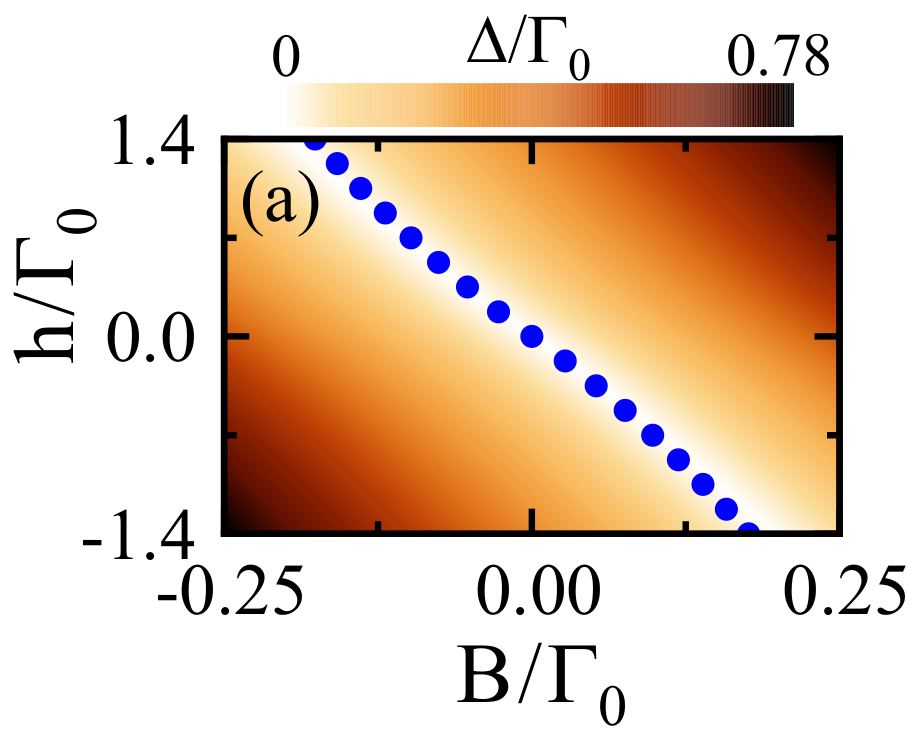
\includegraphics[width=0.55\textwidth]{Bc1.png}
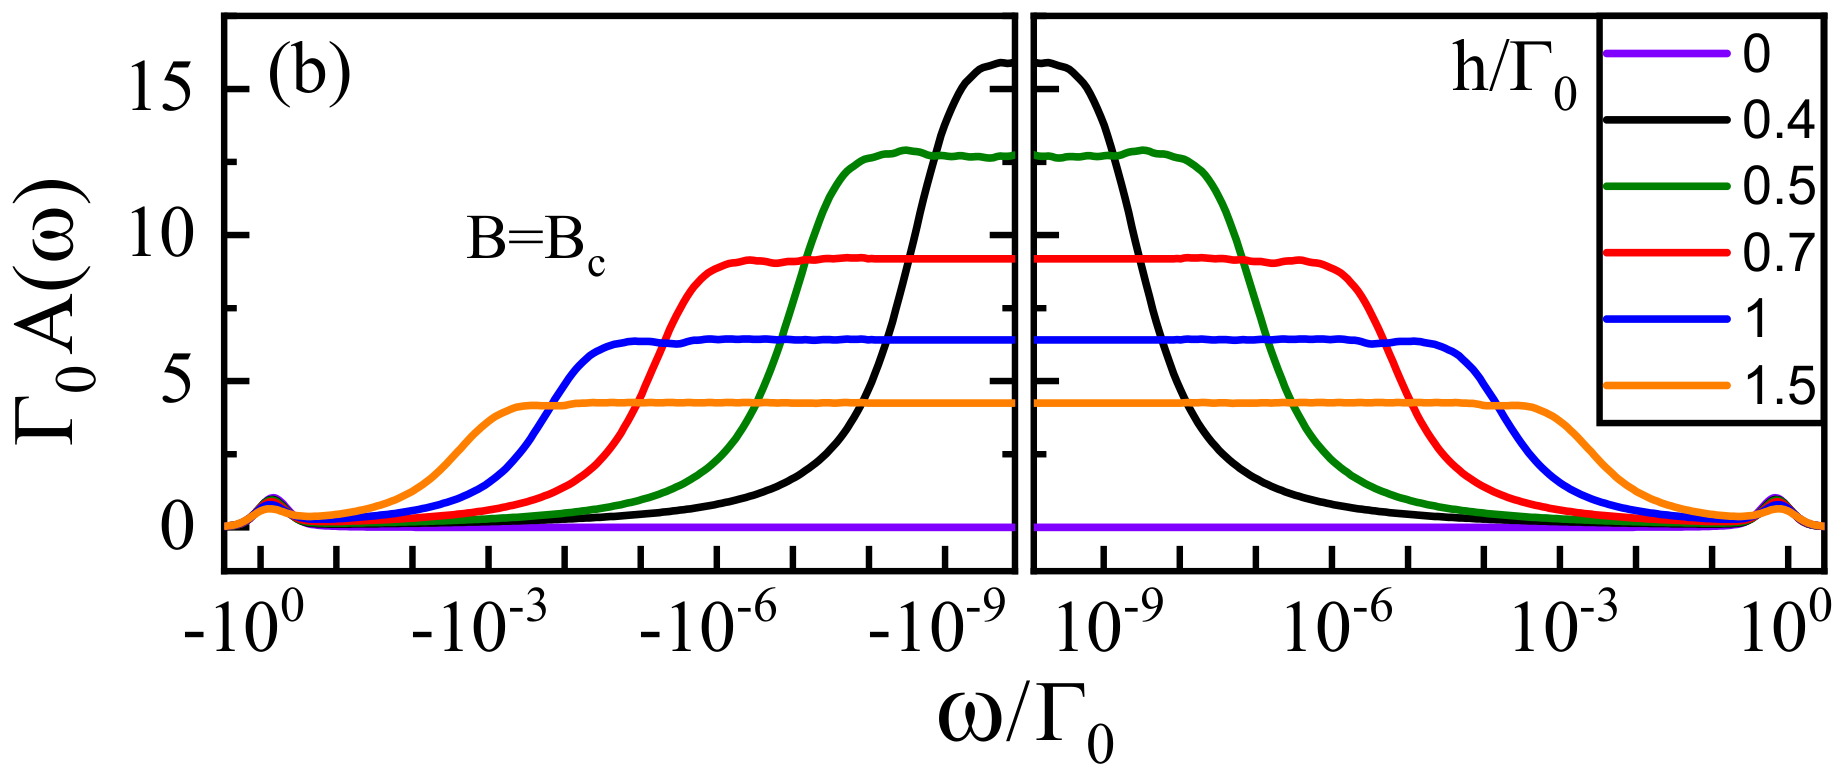
\includegraphics[width=0.94\textwidth]{Aw-h-Bc.png}
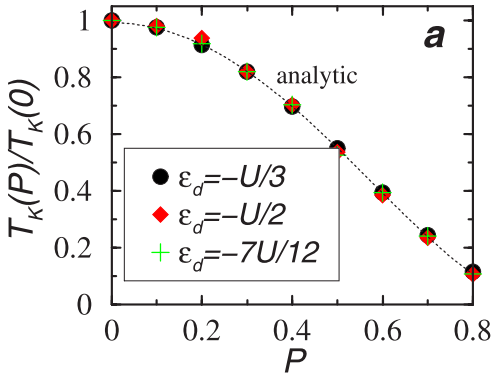
\includegraphics[width=0.45\textwidth]{Tk-P.png}
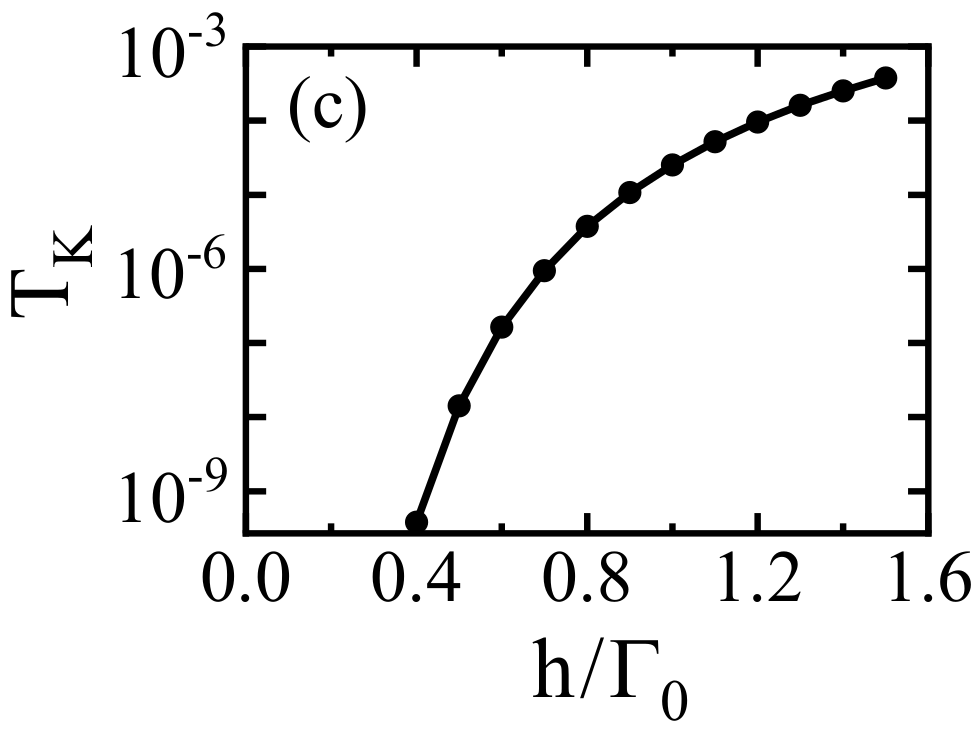
\includegraphics[width=0.45\textwidth]{tk-h.png}
\end{figure}
\end{minipage}
\center{铁磁性增高了近藤温度$T_{k}$!}
\end{frame}

\subsection{2.3受门电压调控的铁磁性诱导的近藤屏蔽}
\title{铁磁石墨烯中近藤效应的NRG研究\qquad \qquad \qquad \qquad 背景}
\begin{frame}{受门电压调控的石墨烯近藤效应}
\begin{figure}
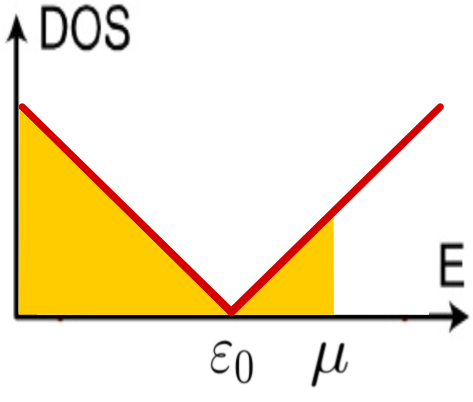
\includegraphics[width=0.3\textwidth]{gated-dos.png}
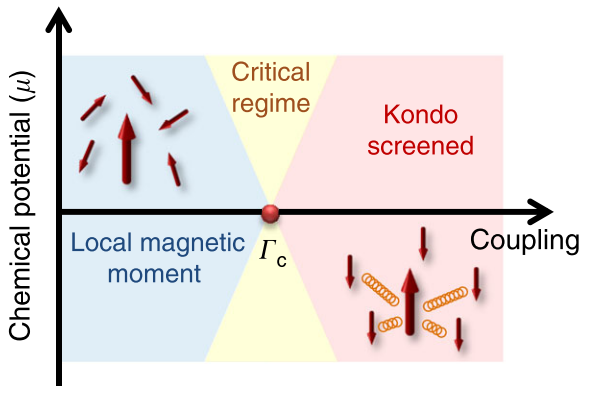
\includegraphics[width=0.35\textwidth]{phasediagram.png}
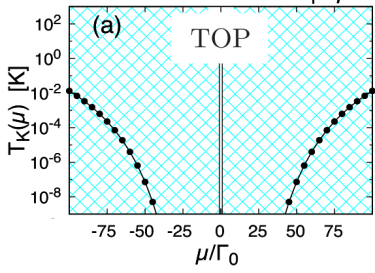
\includegraphics[width=0.32\textwidth]{tk-mu.png}
\end{figure}
\hspace{9cm}PRB \textbf{95}, 115408
\vspace{0.7cm}
\begin{itemize}
\setlength\itemsep{0.4em}
\item 化学势$\mu$可以用来调节打开或关闭近藤效应
\item $\mu$具体对近藤物理的影响,如$T_{k}(\mu), \Gamma_{c}(\mu), n_{\rm{imp}}(\mu)$
\item $\mu$越大,$\rho(\mu)$越大,更有利于近藤屏蔽的形成,近藤温度越高
\end{itemize}
\end{frame}

\title{铁磁石墨烯中近藤效应的NRG研究\qquad \qquad \qquad \qquad 受门电压和铁磁性调控的石墨烯近藤效应}
\begin{frame}{门电压与铁磁性对杂质态密度的影响}
\begin{minipage}[t]{0.45 \textwidth}
参数:
\[U=0.2,\delta=0,\Gamma_{0}=0.1\]
\[\mu\neq 0, h\neq 0, B=0\]
杂化函数:
\[
\Gamma_{\uparrow}(\omega)=\Gamma_{0}\left|\omega-\varepsilon_{0}+\mu- h\right|
\]
\[
\Gamma_{\downarrow}(\omega)=\Gamma_{0}\left|\omega-\varepsilon_{0}+\mu + h\right|
\]
\begin{itemize}
\setlength\itemsep{0.5em}
\item 调节化学势$\mu$后出现了近藤峰
\item 固定$\mu$,增大$h$,抑制近藤共振,与铁磁金属电极相似
\item 固定$h$,增大$\mu$,近藤肩膀$\rightarrow$劈裂的近藤峰
\end{itemize}
\end{minipage}%
\begin{minipage}[t]{0.55 \textwidth}
\begin{figure}
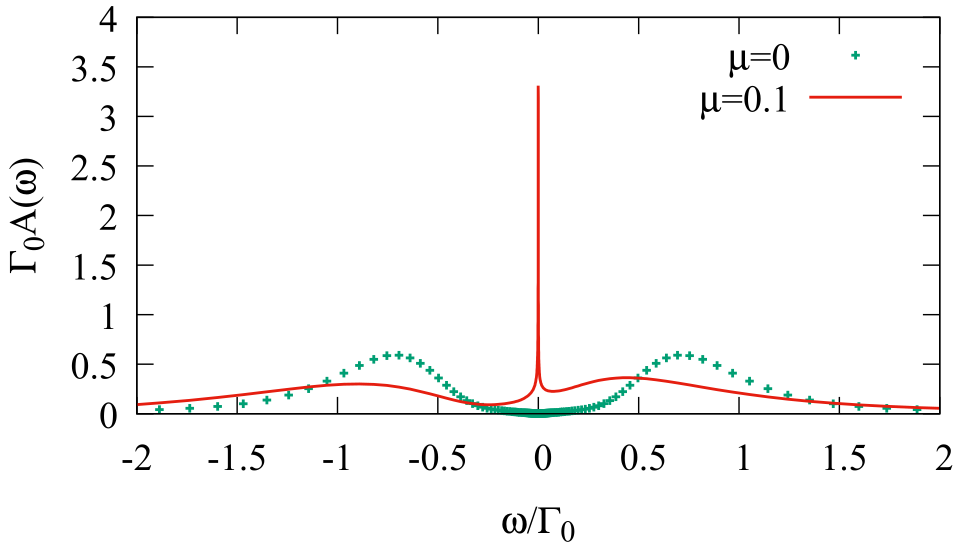
\includegraphics[width=0.97\textwidth]{dos-mu.png}\\
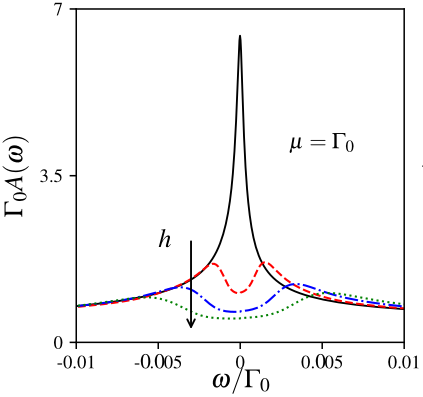
\includegraphics[width=0.49\textwidth]{dos-mu-h2.png}
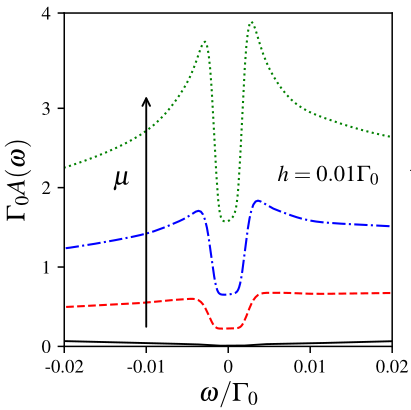
\includegraphics[width=0.49\textwidth]{dos-mu-h1.png}
\end{figure}
\end{minipage}
\end{frame}

\begin{frame}{门电压与铁磁性对近藤温度的影响}
\begin{minipage}[t]{0.45 \textwidth}
参数:
\[U=0.2,\Gamma_{0}=0.4\]
\[\delta=\{0,-0.43\}\]
\[\mu\neq 0, h\neq 0, B=0\]
杂化函数:
\[
\Gamma_{\uparrow}(\omega)=\Gamma_{0}\left|\omega-\varepsilon_{0}+\mu- h\right|
\]
\[
\Gamma_{\downarrow}(\omega)=\Gamma_{0}\left|\omega-\varepsilon_{0}+\mu + h\right|
\]
\begin{itemize}
\setlength\itemsep{0.5em}
\item 温度$T<T^{*}$时,杂质进入自旋单态(近藤单态或自旋极化态)
\item 有效能量$T^{*}$定义:$S_{\rm{imp}}(T)$降为$\frac{1}{2}\rm{ln}2$处的温度
\item $h=0$时,$T^{*}$即为近藤温度$T_{k}$
\item 曲线在$\mu\approx \pm h$处出现极小值
\end{itemize}
\end{minipage}%
\begin{minipage}[t]{0.55 \textwidth}
\vspace{0.3cm}
\begin{figure}
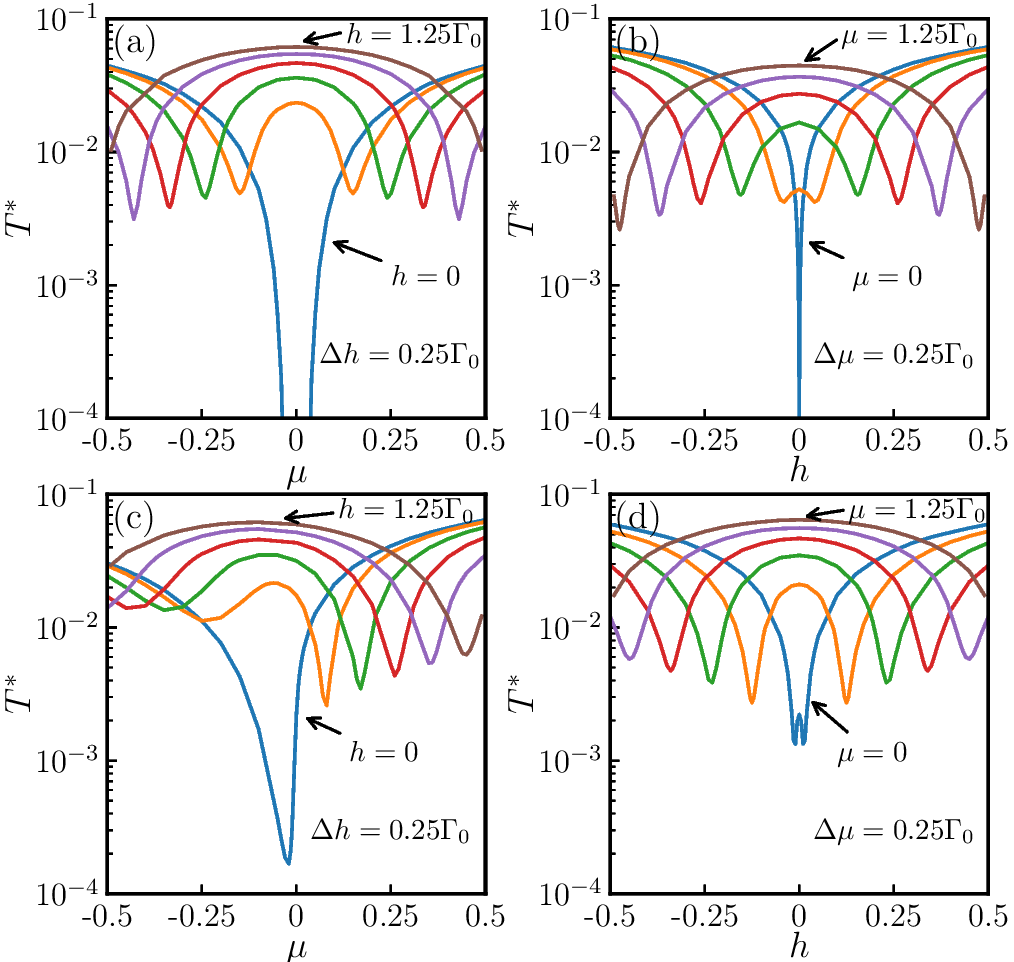
\includegraphics[width=0.9\textwidth]{Tk-mu-h.png}
\end{figure}
\end{minipage}
\end{frame}

\title{铁磁石墨烯中近藤效应的NRG研究\qquad \qquad \qquad \qquad 磁场的补偿?}
\begin{frame}{$\mu\approx h$处的态密度:近藤半金属区}
\begin{figure}
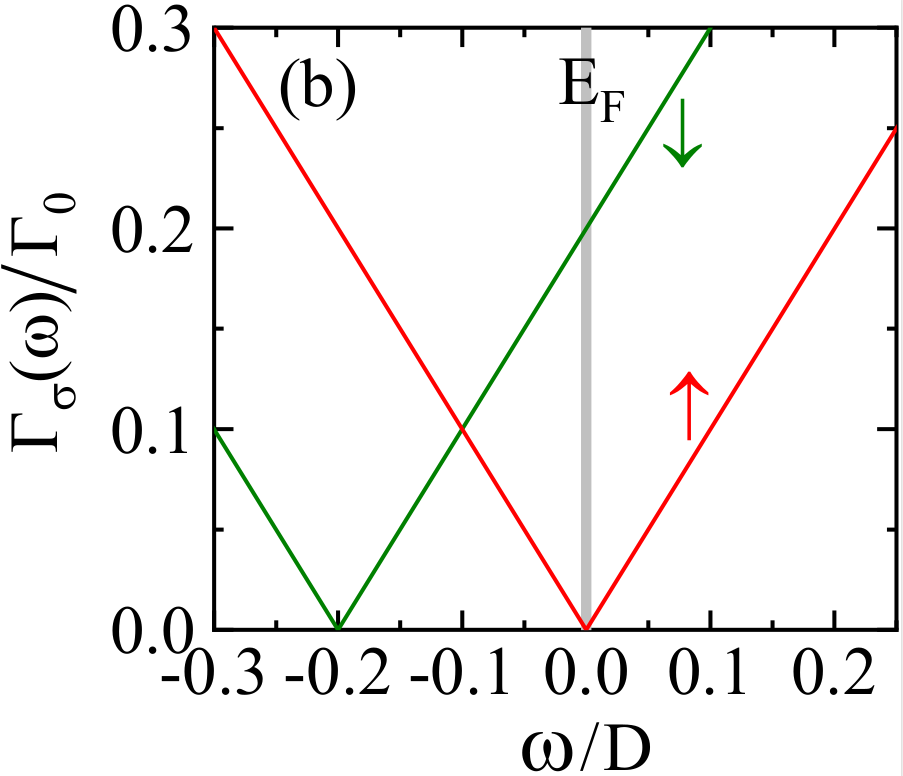
\includegraphics[width=0.28\textwidth,height=0.27\textwidth]{hyb2.png}
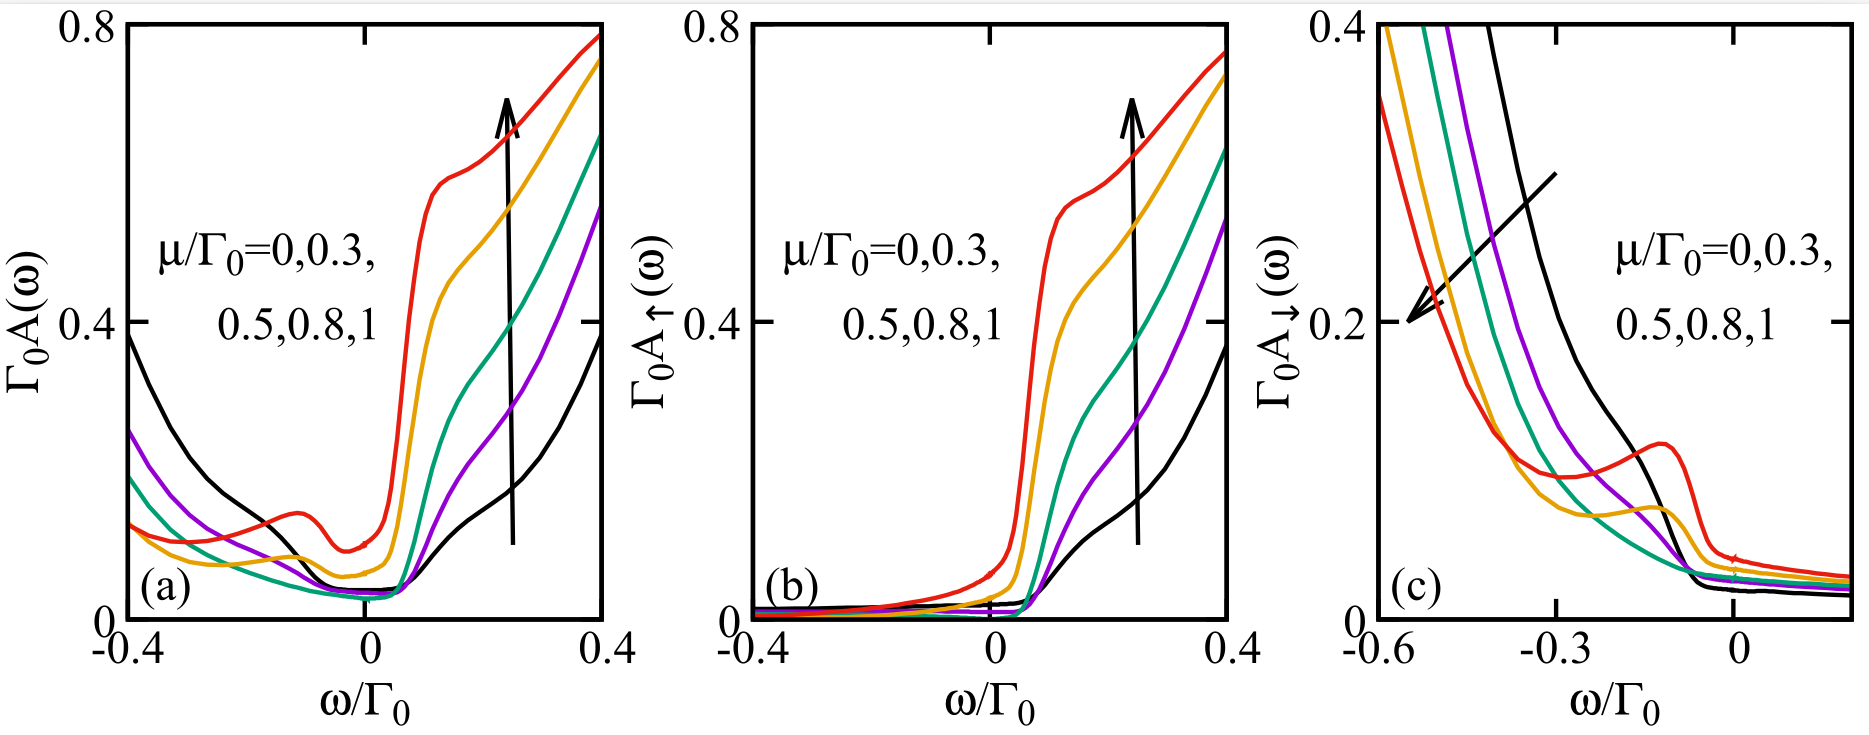
\includegraphics[width=0.7\textwidth]{dos-mu=h.png}
\end{figure}
参数:
\[U=0.2,\delta=0,\Gamma_{0}=0.1\]
\center{$\mu\neq 0$,\framebox[1.1\width]{$h/\Gamma_{0}=0.5,$} $B=0$}
\begin{itemize}
\vspace{0.3cm}
\setlength\itemsep{0.5em}
\item $\mu=h$时,$\rho_{\uparrow}(E_{F})=0$,不能形成近藤共振
\item 只有一个自旋分量的态密度有近藤共振
\item 类似于半金属行为,称为近藤半金属区
\end{itemize}
\end{frame}

\subsection{2.4外磁场对近藤屏蔽的补偿与抑制}
\title{铁磁石墨烯中近藤效应的NRG研究\qquad \qquad \qquad \qquad 近藤半金属}
\begin{frame}{磁场对石墨烯中近藤半金属的显著调节}
\begin{figure}
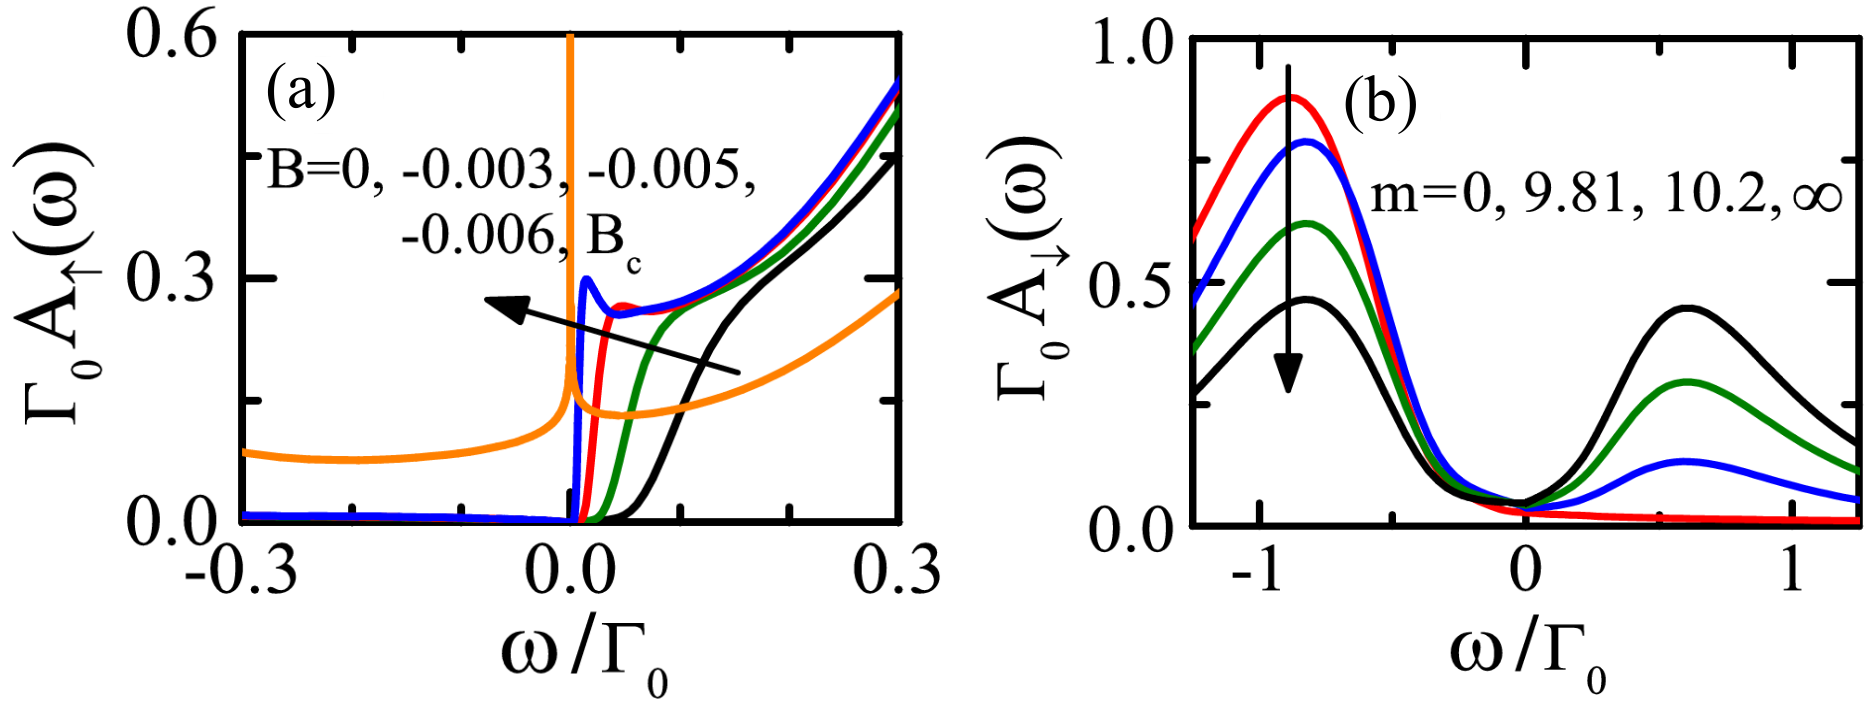
\includegraphics[width=0.55\textwidth ,height=0.25\textwidth]{dos-B.png}
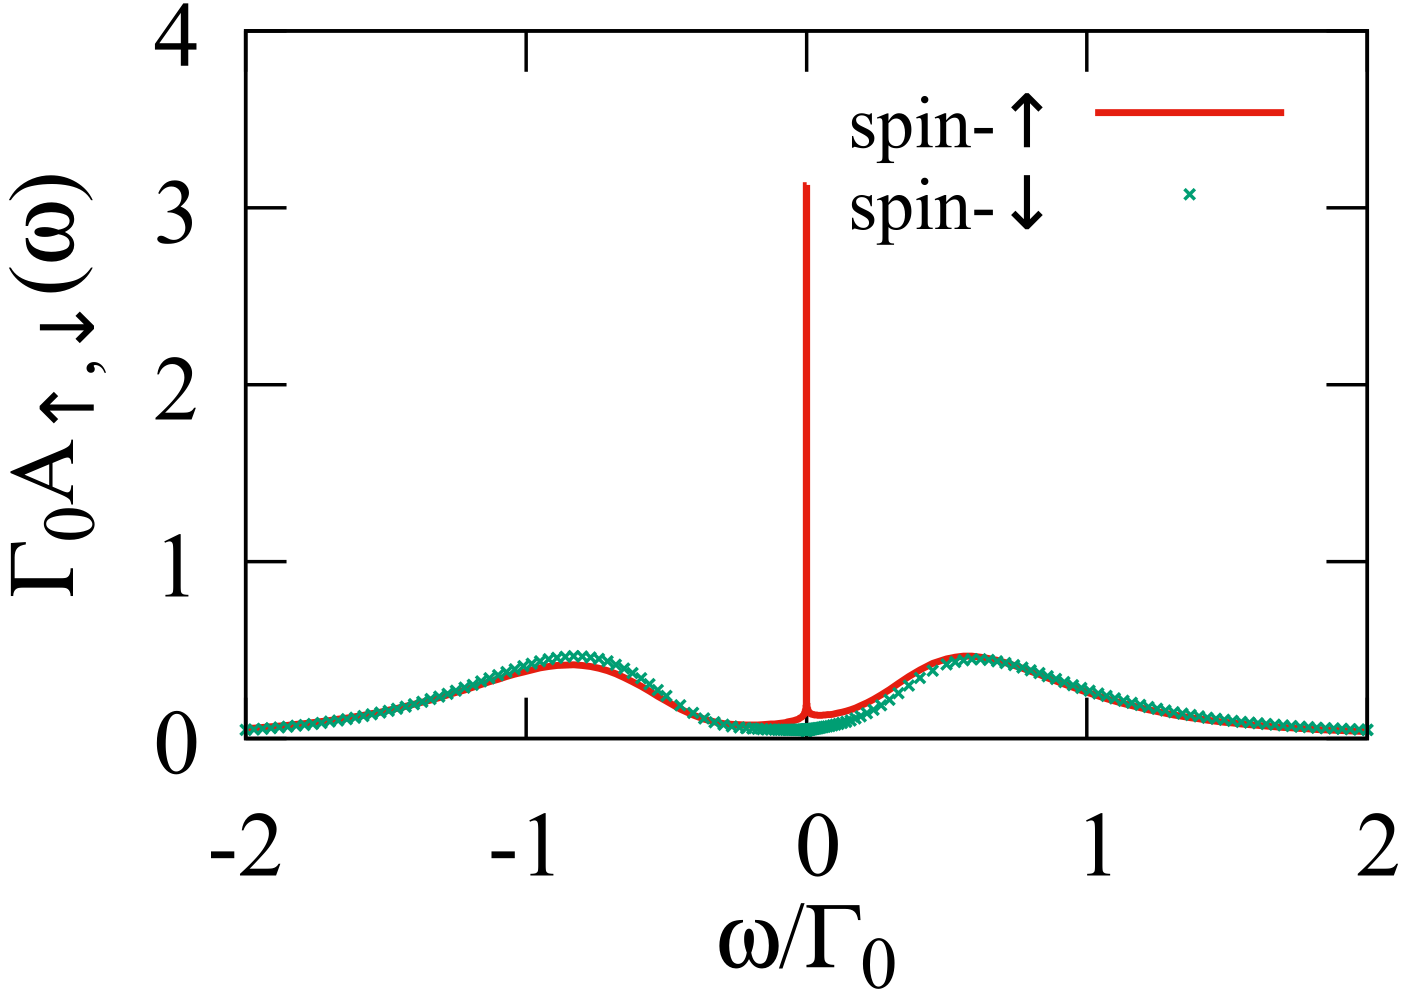
\includegraphics[width=0.35\textwidth,height=0.25\textwidth]{halfmetal.png}
% 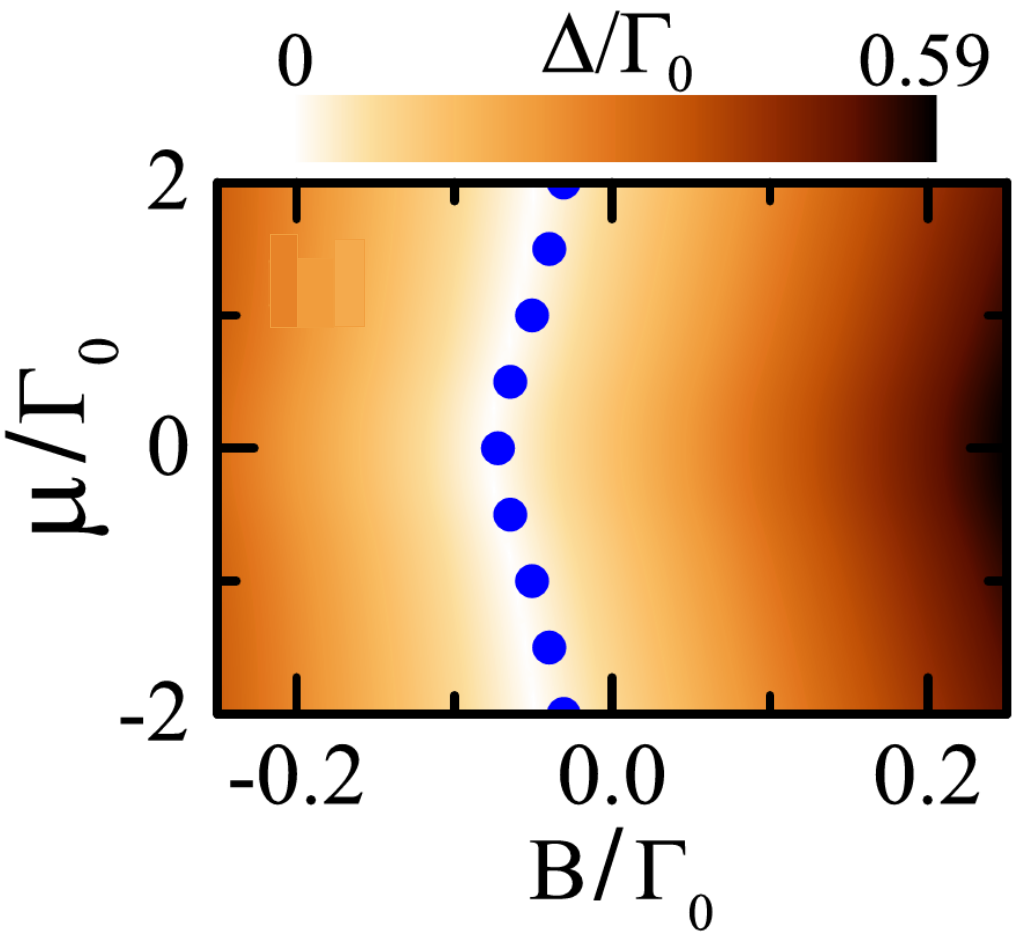
\includegraphics[width=0.18\textwidth,height=0.22\textwidth]{delta.png}
\end{figure}
参数:
\center{\framebox[1.1\width]{$\mu/\Gamma_{0}=h/\Gamma_{0}=0.5,$} $B=B_{c}$}
\begin{itemize}
\vspace{0.3cm}
\setlength\itemsep{0.5em}
\item $B=(1-10^{-m})B_{c}$
\item 被磁场增强的态密度,只有一个自旋分量有近藤峰
\item 不同自旋的不同输运行为,应用意义
% \item 固定$h/\Gamma_{0}=0.5$,临界补偿磁场$B_{c}$对化学势$\mu$的依赖
\end{itemize}
\end{frame}

\subsection{2.5小结}
\title{小结}
\begin{frame}[t]{小结}
\vspace{0.6cm}
\qquad 量子杂质问题是凝聚态物理领域倍受关注的问题,量子杂质问题的研究对多体相互作用的理解如介观输运、纳米器件的制备和工业应用都有重要的作用。

\vspace{0.3cm}
\qquad 我们用FDM-NRG研究了石墨烯中的近藤现象,发现了:
\vspace{0.2cm}
\begin{itemize}
% \setlength\itemsep{0.5em}
\item 在石墨烯中铁磁性可以诱导近藤共振
\item 可以用磁场调节
\item 并发现可以通过调节化学势$\mu$和铁磁性$h$使得石墨烯处于一种状态$\mu=h$
\item 在这种状态下,系统中不同自旋的电子具有不同的输运行为
\end{itemize}

\end{frame}

\section{3.机器学习}

\begin{frame}
\tableofcontents[currentsection] 
\end{frame}

\subsection{3.1机器学习}
\title{机器学习}
% \begin{frame}[t]{数据挖掘的一般流程}
% \begin{figure}
% \centering
% \includegraphics[width=0.3\textwidth]{data-mining.png}
% \includegraphics[width=0.6\textwidth]{data-mining-steps.png}
% \end{figure}
% % \begin{minipage}[t]{0.65 \textwidth}
% 跨学科的计算机科学分支,用人工智能、机器学习和统计学的交叉方法在相对较大型的数据集中发现模式的计算过程。

% 数据挖掘的步骤:
% \begin{itemize}
% \item[1.] 定义问题-确定数据挖掘的目标
% \item[2.] 验证数据-评估、收集、理解数据
% \item[3.] 预处理数据–以使数据中没有噪音或不规则性
% \item[4.] 模型化数据-选择算法以建立预测性模型
% \item[5.] 训练与测试模型-在训练集和测试集上分别对模型进行训练和测试
% \item[6.] 验证与部署-验证模型的范化能力,可视化与部署
% \end{itemize}
% % \end{minipage}%
% % \begin{minipage}[t]{0.33 \textwidth}
% % \end{minipage}\\ $\quad$
% \end{frame}
% \begin{frame}[t]{数据挖掘案例:用户电影评论分析}
% 假设你是Netflix的一名数据分析师,你想要根据用户对不同电影的评分研究用户在电影品位上的相似和不同之处。了解这些评分对用户电影推荐系统有帮助。
% \begin{figure}
% \centering
% % \includegraphics[width=0.3\textwidth]{data-mining.png}
% \includegraphics[width=0.58\textwidth]{movie-clustering.png}
% \end{figure}
% \end{frame}

% \begin{frame}[t]{数据挖掘案例:个人信用评分卡建模}
% \begin{minipage}[t]{0.3 \textwidth}
% \begin{figure}
% \centering
% \includegraphics[width=0.93\textwidth, height=0.8\textheight]{credit2.png}
% \end{figure}
% \end{minipage}%
% \begin{minipage}[t]{0.68 \textwidth}
% \begin{figure}
% \centering
% \includegraphics[width=0.93\textwidth]{credit1.png}
% \end{figure}
% 张三的信用评分: 
% \[223\text{\tiny{(基准分)}} + 8\text{\tiny{(年龄)}} + 4\text{\tiny{(性别)}} + 8\text{\tiny{(婚姻状况)}} + 8\text{\tiny{(学历)}} + 13\text{\tiny{(月收入)}} = 264\]
% 信用评分卡建模就是建模得出各个得分的过程。
% \end{minipage}
% \end{frame}

\subsection{3.2深度学习算法}
\begin{frame}[t]{深度学习算法}
\begin{minipage}[t]{0.3 \textwidth}
\vspace{0.1cm}
\begin{itemize}
\item 多层感知器MLP
\item 卷积神经网络CNN
\begin{itemize}
\item[-] AlexNet(2012)
\item[-] VGGNet(2014)
\item[-] GoogleNet(2014)
\item[-] ResNet(2015)
% \item[-] ...
\end{itemize}
\item 循环神经网络RNN
\begin{itemize}
\item[-] LSTM(1997)
\item[-] GRU(2014)
% \item[-] ...
\end{itemize}
\item 生成对抗网络GAN
\begin{itemize}
\item[-] DCGAN
\end{itemize}
\end{itemize}
\vspace{0.1cm}
目前存在问题:
\begin{itemize}
\setlength\itemsep{0.03em}
\item[-] 训练时间长(分布式训练)
% \item[-] 梯度消失问题(ReLU, BN, 跳连接)
\item[-] 超参太多
\item[-] 解释性差
\end{itemize}

\end{minipage}%
\begin{minipage}[t]{0.68 \textwidth}
\begin{figure}
\centering
\includegraphics[width=0.98\textwidth]{DL-history.png}\\
\tiny{《深度学习综述》,张荣(2018)}
\end{figure}
\begin{minipage}[t]{0.5 \textwidth}
\textbf{应用:}
\begin{itemize}
% \item[-] 语音处理
\item[-] 计算机视觉
\item[-] 自然语言处理
\end{itemize}
\end{minipage}%
\begin{minipage}[t]{0.5 \textwidth}
\begin{itemize}
% \setlength\itemsep{0.1em}
\setlength\itemsep{0.03em}
% \item[-] 生物信息学
\item 模型$\rightarrow$参数$\rightarrow$最大似然估计$\rightarrow$ 最优化
\end{itemize}
\end{minipage}
\end{minipage}
\end{frame}

\subsection{3.3神经网络的分布式并行训练}
\begin{frame}[t]{案例:用对抗生成网络学习手写数字}
\vspace{-0.54cm}
\begin{minipage}[t]{0.6 \textwidth}
\begin{figure}
\centering
\includegraphics[width=\textwidth]{GAN.png}
\ \\
\includegraphics[width=0.4\textwidth]{real-digit.png}
\end{figure}
\end{minipage}%
\begin{minipage}[t]{0.4 \textwidth}
\begin{figure}
\centering
\includegraphics[width=\textwidth, height=0.9\textheight]{generated-digit.png}
\end{figure}
\end{minipage}
\textcolor{red}{结论}:无论单节点还是多节点都建议使用DistributedDataParallel方法,甚至分布式训练的方式比单个节点上多GPU的训练方式更高效。
\end{frame}
\begin{frame}[t]{神经网络的分布式并行训练}
\begin{minipage}[t]{0.3 \textwidth}
\vspace{0.3cm}
分布并行训练的方式:
\begin{itemize}
\setlength\itemsep{0.1em}
\item[-] \textcolor{red}{数据并行}
\item[-] 模型并行
\item[-] 混合并行
\end{itemize}
并行加速比: 
\[ S_p = T_1 / T_p \]
并行加速效率:
\[ E_p = S_p / p = T_1 / pT_p \]
$p$为GPU个数,$T_p$为程序在$p$个GPU上运行的时间。
\end{minipage}%
\begin{minipage}[t]{0.7 \textwidth}
\begin{figure}
\centering
\includegraphics[width=\textwidth]{time-consumption.png}
\caption{Pytorch内置的DistributedDataParallel并行实现,多节点GPU通信后端为NCCL。}
\end{figure}
\end{minipage}
\textcolor{red}{结论}:无论单节点还是多节点都建议使用DistributedDataParallel方法,甚至分布式训练的方式比单个节点上多GPU的训练方式更高效。
\end{frame}
\section{4.机器学习+量子多体计算}
\title{}
\begin{frame}{}
\vspace{0.25\textwidth}
% \frametitle{}
\center{\Large{机器学习+量子多体计算=?}}
\end{frame}

\section{5.致谢}
\title{}
\begin{frame}{}
\vspace{0.25\textwidth}
\frametitle{致谢}
\center{\Large{感谢各位评委老师!}}
\end{frame}

\end{document}
